\documentclass[a4print,english,lof,lot]{univpmphdthesis}
\errorcontextlines=9

\RequirePackage[utf8]{inputenc}
\RequirePackage[T1]{fontenc}

\usepackage{lmodern}
\usepackage[cmex10]{amsmath}
\usepackage{amssymb}
\usepackage{subcaption}
\usepackage{multirow}
\usepackage{booktabs}
\usepackage{framed}
\usepackage{algorithm,algpseudocode}
\usepackage[table,xcdraw]{xcolor}
\usepackage{pgfplots,pgfplotstable}
\usetikzlibrary{pgfplots.groupplots}
\usepackage{tabularx}

\usepackage{tikz}
\usetikzlibrary{shapes,arrows}

\usepackage{tkz-kiviat,numprint}
\usetikzlibrary{decorations.pathreplacing, arrows, fit}
\usepackage{hyperref}
%\usepackage{lineno}

\usepackage{collcell}
\usepackage{hhline}
\usepackage{tablefootnote}
\usepackage{siunitx}

\usetikzlibrary{shadows,arrows,fit,shapes,positioning,calc,backgrounds,spy,decorations.markings}
\usetikzlibrary{backgrounds}

\pgfdeclarelayer{background}
\pgfdeclarelayer{foreground}
\pgfsetlayers{background,main,foreground}

\tikzstyle{bk} = [draw, fill=blue!30, text centered, minimum height=2em, text width=7em, minimum width=6em, minimum height=3em, rounded corners, drop shadow]
\tikzstyle{bkFull} = [draw, fill=blue!30, text centered, minimum height=2em, text width=15em, minimum width=20em, minimum height=3em, rounded corners, drop shadow]
\tikzstyle{bkDec} = [draw, fill=red!40, text centered, minimum height=2em, text width=15em, minimum width=15em, minimum height=3em, rounded corners, drop shadow]
\tikzstyle{cy} = [draw, fill=gray!30, text centered, minimum height=3em, text width=7em, minimum width=2em, cylinder, shape border rotate=90, shape aspect=0.1, drop shadow]
\tikzstyle{cyFull} = [draw, fill=gray!30, text centered, minimum height=3em, text width=7em, minimum width=20em, cylinder, shape border rotate=90, shape aspect=0.1, drop shadow, dashed]
\tikzstyle{bg}=[rectangle,fill=gray!30,inner sep=0.2cm,rounded corners,draw=black!50, dashed]
\tikzstyle{input} = [coordinate]

\tikzset{
	myarrow/.style={
		draw,thick,
		single arrow,
		%text width=1cm,
		minimum height=1cm,
		%anchor=west,
		%fill=white
	},
}

\tikzstyle{vecArrow} = [thick, decoration={markings,mark=at position 1 with {\arrow[semithick]{open triangle 60}}},
double distance=1.4pt, shorten >= 5.5pt, preaction = {decorate}, postaction = {draw,line width=1.4pt, white,shorten >= 4.5pt}]

\tikzstyle{innerWhite} = [semithick, white,line width=1.6pt, shorten >= 4.5pt]




\newcommand{\LegendBox}[3][]{%
	\xdef\fitbox{}%
	\coordinate[#1] (LegendBox_anchor) at (#2) ;
	\foreach \col/\item [count=\hi from 0] in {#3} {
		\node[color = \col,draw,thick,
		fill  = \col,
		minimum width  = 5 ex,
		minimum height = 1 ex,
		name=b\hi,
		] at ([yshift=0 ex,xshift=\hi*40 ex]LegendBox_anchor) {};
		\node[anchor=west,xshift=0.1 ex] at (b\hi.east) (c\hi) {\item};
		\xdef\fitbox{\fitbox(c\hi)}
	}%
	\node [fit=\fitbox(LegendBox_anchor), minimum width = 0 ex] {};
}


\newcommand{\chref}[1]{Chapter~\ref{#1}}
\newcommand{\secref}[1]{Section~\ref{#1}}
\newcommand{\subsecref}[1]{Subsection~\ref{#1}}
\newcommand{\paragref}[1]{Paragraph~\ref{#1}}

\newcommand{\apxref}[1]{Appendix~\ref{#1}}

\newcommand{\figref}[1]{\figurename~\ref{#1}}
\newcommand{\tableref}[1]{Table~\ref{#1}}
%\newcommand{\eqref}[1]{Equation~\ref{#1}}

\newcommand*\rfrac[2]{{}^{#1}\!/_{#2}}


\def\N{{\mathbb{N}}}
\def\Z{{\mathbb{Z}}}
\def\R{{\mathbb{R}}}


% Il codice che segue colora una cella in base al suo contenuto
% #1 è il contenuto della cella (ad esempio, 80)
% \pgfmathparse{#1/100<.7?1:0} 

\newcommand\gray{gray}
\newcommand\ColCell[1]{%
	\pgfmathparse{#1/100<.7?1:0}% valuta se #1/100 è maggiore di 0.7 oppure è minore. Se minore ritorna 1, altrimenti 0
	\ifnum\pgfmathresult=0\relax\color{white}\fi % imposta il colore del testo a bianco se il risultato di pgfmathparse è 0
	\pgfmathparse{1-#1/100}% calcola 1-#1/100
	\expandafter\cellcolor\expandafter[%
	\expandafter\gray\expandafter]\expandafter{\pgfmathresult}#1} % colora la cella della gradazione di grigio impostata dal risultato di pgfmathparse ed inserisce il valore originario della cella.
\newcolumntype{E}{>{\collectcell\ColCell}c<{\endcollectcell}}
\newcolumntype{K}[1]{>{\centering\arraybackslash}p{#1}}
%\modulolinenumbers[5]

%%%%%%%%%%%%%%%%%%%%%%%%%%%%%%%%%%%%%%%%%%%%%%%%%%%%%%%%%%%
% Metadata
%%%%%%%%%%%%%%%%%%%%%%%%%%%%%%%%%%%%%%%%%%%%%%%%%%%%%%%%%%%
\phdschool{Scuola di Dottorato di Ricerca in Scienze dell'Ingegneria}
\phdfaculty{Facolt\`{a} di Ingegneria}
\phdcurriculum{Curriculum in Ingegneria Elettronica, Elettrotecnica e delle Telecomunicazioni}
\phdtitle{Ambient Intelligence: Computational Audio Processing For Human Fall Detection}
%\phdsubtitle{con questa bellissima classe} % NON NECESSARIO
\phdauthor{Diego Droghini}
\phdadvisor{Prof.~Francesco Piazza}
\phdcoadvisor{Prof.~Roberto Bedini} % IN TEORIA NON E' AMMESSO
%\phdcoadvisor{Prof.~Michele Blu} % IN TEORIA NON E' AMMESSO
\phdcurriculumadvisor{Prof.~Francesco Piazza}
\phdcycle{17}
\thesisdedication{alla mia famiglia}
\phdlocation{Ancona}
\phdtime{Ottobre 2018}
%%%%%%%%%%%%%%%%%%%%%%%%%%%%%%%%%%%%%%%%%%%%%%%%%%%%%%%%%%%

% Solo per generare testo...
\usepackage{lipsum}

\begin{document}

%%%%%%%%%%%%%%%%%%%%%%%%%%%%%%%%%%%%%%%%%%%%%%%%%%%%%%%%%%%
% Front matter contents
%%%%%%%%%%%%%%%%%%%%%%%%%%%%%%%%%%%%%%%%%%%%%%%%%%%%%%%%%%%
\frontmatter

\maketitle

%\begin{thesisacknowledge}
%\lipsum[1-2]
%\end{thesisacknowledge}

%\begin{thesisacknowledge}[italian]
%\lipsum[1-2]
%\end{thesisacknowledge}

\begin{thesisabstract}
\lipsum[1-3]
\end{thesisabstract}

\thesistoc

%%%%%%%%%%%%%%%%%%%%%%%%%%%%%%%%%%%%%%%%%%%%%%%%%%%%%%%%%%%
% Main matter contents
%%%%%%%%%%%%%%%%%%%%%%%%%%%%%%%%%%%%%%%%%%%%%%%%%%%%%%%%%%%
\mainmatter

\graphicspath{{1_introduction/}}
\chapter{Introduction}\label{ch:intro}


Ambient intelligance + computation audio processing + obiettivi, controbuti, Outline

 The origins of the Ambient Intelligence are rooted in the birth of domotics and Home Automation. In fact, the concept of home automation design was already being started in the 80s for residential buildings. the information revolution, microprocessors and telecommunication networks are the main elements that have allowed the development of domotics. At the same time, increasingly sophisticated automation processes in the manufacturing field are at the base of building automation and domotics applications, transferring the control and automation systems present in the factories, with appropriate measures, to the building and its plants. During the decade '70 '80 the foundations for the transformation of household appliances were laid. In this phase, we witness the first transition from the electric house to the electronic house; subsequently, the progress of the sector will lead to the current concepts of integrated home system, and therefore bringing with it the concept of services that put man at the centre, and therefore of \textit{ambient intelligence}. The vision of the Ambient Intelligence (AmI) \cite{ducatel2001scenarios} has its foundations in the article M. Weiser \cite{weiser1991}. He states that ``the deepest technologies are those that disappear'' and states that computer technology at the time of its maturity should be invisible.
 Today the efforts in this direction are aimed at creating a ``non-deterministic and open'' cyberspace within which autonomous and intelligent entities will interact in order to put man at the centre of a design that will see the realisation of the fully integrated home of the future. This space will be able to self-organise and self-adapt to the user and anticipating his needs. The systems that conform to this vision will offer technological solutions that will be integrated into the environment, context-aware, tailored to the user need, able to adapt actions in new scenarios, able to anticipate the needs and wishes of users, all with minimal user intervention. 
 The objects and the environment will interact with each other in order to support users in carrying out their daily activities in a natural way, using the information and the intelligence that is hidden in the technological infrastructure that connects the devices (the technological complexity will become invisible for the user).
 In an AmI system, many heterogeneous devices work in cooperation to support users in everyday activities. As a result, the intelligence has been introduced in the domestic environment to provide more comfortable spaces for the inhabitants and allow the automatic implementation of different functions, such as ensuring greater independence and autonomy of the inhabitants acting in the areas of security/safety and issues of Ambient Assisted Living (AAL). A particular its application to the field of AAL is precisely the human fall detection. 
 
The decreasing birth rate \cite{eurostat} and the contemporary increase of the life expectancy at birth \cite{Carone2006} in the majority of industrialized countries have been generating new challenges in the assistance of the elderly. The scientific community, companies and governments are trying to face them by investing in the development of efficient healthcare systems and solutions. The direction taken goes towards the development of smart home capable of taking care of the inhabitants by supporting and monitoring them in their daily actions \cite{Dawadi20161188, Principi2015a}. Since falls are one of the main cause of death for the elderly \cite{mubashir2013survey}, several efforts have been devoted to the development of algorithms for automatically detecting these events.
This work is aimed at the presentation of different computational audio processing systems for fall detection. The approach described in each chapter follow a data available perspective. 

INSERIRE CONTRIBUTI E OBIETTIVI

The outline of the dissertation is the following.
\secref{sec:fds} introduce the human fall classification task with an update state of the art of the approaches mainly related to those that are audio based. \chref{ch:backg} gives an overview of the theoretical background of the data-driven techniques used in the presented approaches. The \chref{ch:dataset} described the dataset made by the authors, used for the assessment of the systems. \chref{ch:supervised_approaches} presents the supervised approaches aimed to evaluate both the created dataset and the proposed innovative sensor.
The unsupervised system are described in \chref{ch:unsupervised_approaches} where no human fall data has been used to train the algorithms.
In \chref{ch:weakley_supervised} approaches that operate in more realistic conditions are described.





\section{Fall Detection Systems}
\label{sec:fds}
The continuous and unprecedented growth rate of the elderly world population is one of the primary aspects of concern for society and governments. Nowadays about 8.5\% of people in the world are more than 65 years old \cite{dhhsOlderPop,Carone2006}. Although the average life of the world population is getting longer, elderly people may not    necessarily live a healthier life. It is enough to say that 37.5 million falls require medical interventions and more than 600 thousand are cause of death every year worldwide. In particular, the population segment most affected by this problem is composed of elderly over 65 years that, with the growing mobility of the population, are more frequently left alone in their homes without aid in the case of need. Moreover, since falls are the leading cause of death and hospitalizations for older adults, this phenomenon leads to a substantial increase in the cost of healthcare \cite{whoFall, mubashir2013survey}. 
It is not surprising, thus, that the research community is encouraged, even by governments, to find reliable and performing solutions to minimize the damage caused by the human falls problem. This is also confirmed by the presence in the literature of several reviews dedicated to this specific topic \cite{mubashir2013survey, khan2017review, lapierre2017state, pannurat2014automatic, xu2018new, el2013fall}.
In fact, in the past few years, a variety of systems have been presented. One way to divide the methodologies for approaching the falls detection problem is based on the placement of the sensing devices \cite{mubashir2013survey}. The main categories are wearable, vision and environmental, with each category presenting their own advantages and disadvantages. Wearable systems do not suffer from ambient condition, but people may forget to wear them and they are not operational during the charging time, thus, some people may consider them annoying. Furthermore, a device must be installed on each person to be monitored. An environmental sensor may be used to avoid this kind of problems, but with other limitations. Vision systems, although they are actually environmental sensors, deserve a dedicated category because of many systems proposed in the literature based on this type of sensors \cite{mubashir2013survey}. This category includes several types of sensors like, e.g., cameras for which the major limitations are field-of-view constraints, lighting condition, positioning of multiple cameras and lack of privacy.
The ambient category includes several types of sensors. For example, radar doppler based systems used in \cite{wu2015radar} raise fewer privacy concerns, but they suffer from reflection and blind spots. In particular, for a data-driven system, another aspect that should not be underestimated is the need for a re-training when changing the environment to be monitored or even just some of its components such as the arrangement of furniture as happens in \cite{liu2008vision}.
All this implies that there is no optimal choice, which is instead, a compromise that depends on the type of environment that is monitored as well as on personal sensitivity of the subjects under monitoring.
Going into more detail, another significant distinction between falls detection systems can be made based on the type and amount of data used for the algorithm development \cite{khan2017review}. In fact, the problem can be approached either as supervised or unsupervised based on the availability of data in the hands of the researchers as well as their goals. 
Most state-of-the-art works tackle the problem under fully supervised conditions assuming they have enough data for falls. Almost all of these falls are simulated with professional mannequins \cite{werner2011fall, zigel2009method}  or by people with adequate protections \cite{li2012microphone, popescu2008acoustic} that however may not correctly emulate an actual fall. Although this approach leads to more accurate results, there is no guarantee that it will generalize well in real situations. 
Other researchers opt for approaches based on outlier/anomaly detection \cite{khan2015unsupervised, zhang2009detecting, popescu2009acoustic} because of the plentiful availability of data that can represent normal activity. However, it is challenging to define what ``normal activities'' are for such approaches, and the risk is to raise several false alarms. % come succede a noi con la ocsvm.
Perhaps the situation that most closely approximates reality is a hybrid between the previous ones, in which a large amount of data representing the normality are easily available, with just a few samples of real human fall (\textit{RHF}) and eventually some related synthetic or simulated data. In these situations, supervised approaches that suffer from strong data imbalance have to apply subsampling \cite{stone2015fall} or weighting \cite{khan2017review} techniques to mitigate this effect. Thus, the need to find an effective way to exploit the few available falls data is evident.

\section{State-Of-The-Art} 
\label{sec:soa}
Review dei sistemi per la fall detection basati sui vari tipi di sensori
accelerometers, vision, ambient. Per gli ambient paricolare enfasi sugli approcci basati su aduio.

As aforementioned, fall detection approaches can be divided based on their sensing technology, in particular if they employ wearable or ambient sensors. Regarding the first ones, the most common choice is to employ accelerometers. The algorithms proposed in \cite{Bourke2007} and \cite{Charlon2013} detect a fall by verifying if the acceleration signals exceed a certain threshold. In contrast, in \cite{Ozdemir2014} the authors implemented several machine learning techniques and studied their classification performance. For the experiments, a fall events dataset has been developed using six sensor units with three-axis accelerometers and worn by 14 persons who simulated falls from different angles. The best performing classifier resulted the $k$-Nearest Neighbour classifier. \cite{Lustrek2015} employed radio tags worn on the user's chest, waist, and ankles, and an optional three-axial accelerometer worn on the chest. The algorithms performs a basic activity recognition, distinguishing from walking, standing, sitting, sitting on the ground, lying down, the process of sitting or lying down, the process of standing up, and falling. The actual fall is detected combining the results of two classifiers, an SVM and a decision tree, and hand-crafted rules. The authors performed the experiments on a laboratory scenario and reported accuracies of 100\% combining radio tags and the accelerometer.

%\cite{lai2011detection}

Differently from wearable sensors, the physical quantities captured by ambient sensors are more heterogeneous. Generally, fall detectors are based on vibration, video or acoustic sensors, sometimes in combination with presence detectors.  In \cite{alwan2006smart} the fall detector is based on a floor vibration sensor and the algorithm detects a fall when the vibration pattern matches the one of a human fall. The authors do not give further details on the algorithm and report 100\% sensitivity and specificity on tests conducted on a dummy falls dataset. Yazar and colleagues \cite{Yazar2013} employ both passive infrared (PIR) sensors and floor vibration sensors. PIRs are employed to reduce false alarms, i.e., by detecting if a person is present in the region of interest. Single-tree complex wavelet transform features are extracted from the vibration signal and classified as fall or non-fall. In their dataset, the non-fall classes are represented by human (walking or running and sitting) or non-human activities (door slamming and a book falling). Three different classifiers have been compared: Euclidean distance, Mahalanobis distance and SVM, with the latter resulting in the most performing one, since it is able to classify human falls without errors regardless the employment of PIR sensors.

Regarding approaches based on audio signals, a common solution is to install several microphones in the building, usually on the ceiling or near the walls. Indeed, also single-microphone approaches exist but they are much less robust to environmental noise, thus resulting in poor performance. For example, in \cite{zhuang2009acoustic}, the authors employ a single far field microphone and they model audio segments by means of perceptual linear predictive (PLP) coefficients and GMM supervectors. An SVM with a kernel based on the Kullback-Leibler divergence, then, classifies the segment as being a fall or noise. For this purpose, nine classes of noise have been considered. In the experiments, the algorithm achieves an F$_1$-Measure of 67\% in the classification task, and an accuracy equal to 64\% in the detection task. 

The difficulty in using a single microphone drove the scientific community to employ multi-channel algorithms. In \cite{khan2015unsupervised} the authors present an unsupervised algorithm based on two microphones. The algorithm comprises a source separation and localization block to reduce the impact of background noise. Then, a one class Support Vector Machine is trained on MFCCs of non-fall events only. The SVM is then applied to distinguish normal sound events (i.e., sounds originating from normal activities) from abnormal ones (i.e., falls sounds). The authors validated the algorithm using simulated falls of persons only in presence of a television that produced the interfering sound. The results in terms of Area Under Curve are 0.9928 without interference and 0.9738 with 75\% interference. The work by Li and colleagues \cite{li2012microphone} employs a circular microphone array to firstly determine the position of the sound source, and then to enhance the signal by applying a beamformer. The height of the sound source is used as first filter to discriminate falls from non falls. If the sound originates from a source positioned on the ground, MFCC features are extracted and a $k$-Nearest Neighbour classifier is employed to detect persons' falls. The algorithm has been tested on a dataset composed of 120 simulated fall sounds and 120 non-fall sounds recorded in different acoustic conditions. In presence of background noise and TV interference, the resulting AUC was equal to 0.989 (accuracy 95\%) on clean conditions and 0.932 at 10\,dB SNR (accuracy 89\%). 

An approach to improve the performance of fall detection systems is to combine the information coming from different sensors. The approach proposed by Zigel \textit{et al.} \cite{zigel2009method} is based on a combination of sound and vibration sensors attached to the floor with a adhesive tape. The algorithm employs energy features extracted from the vibration signal to detect the fall event. Then, the event is classified as fall or non-fall with naive Bayes classifier employing features from both the vibration and sound signals. The experiments were conducted on a dataset containing falls of the ``Rescue Randy'' human mimicking doll and four objects, and the resulting sensitivity and specificity were respectively 97.5\% and 98.6\%. \cite{Liu2014} fuse the information coming from a Doppler sensor and motion sensors and classify falls with an SVM. The authors report an AUC equal to 0.98 with Doppler sensor only, and a further reduction of false alarms by 63\% employing motion sensors information. Motion, sound and video signals are employed in \cite{Doukas2011}. Signals are captured both from environment sensors and from body sensors. A fall is detected by analysing sounds and motion information, while visual and motion behaviour indicates the severity of the fall. The work by Toreyin and colleagues \cite{Toreyin2008} combines PIRs, microphones and vibration sensors. Signals are processed to extract features in the wavelet domain and and HMM classifier is then employed to detect falls. The authors showed the using PIR signals 100\% accuracy can be obtained.

\section{Case studies}
Generally speaking, the ``analytical methods'' distinguish between fall and non-fall events by applying a threshold directly on the acquired signals or on the features sequences extracted from them \cite{noury2007fall}.
These methods are generally built exploiting some a-priori knowledge to operate in a specific scenario and needs manual tuning of the hyperparameters of the algorithm. For these reasons, the ``analytical methods'' can hardly perform when the operating conditions and the subjects are variable. In ``machine learning'' methods, the algorithm learn from the data how to discriminate falls from non-falls \cite{noury2007fall}. Between them can be distinguished ``supervised'' and  ``unsupervised'' approaches. The fist  require a labelled dataset for training the classifier, while the latter build a normality model considering only the non-fall events. Regardless of the used approach, machine learning tasks require that the inputs are mathematically and computationally convenient to process, so researchers have traditionally relied on a two-stage strategy: some features are extracted from the raw signals of dataset and are then used as input for the successive tasks. The choice and design of the appropriate features requires considerable expertise about the problem and constitutes a significant engineering effort.

In this work, different application of computational audio processing based on machine learning techniques for ambient intelligence are analyzed. Particular attention was given to the condition of knowledge for each proposed approach. In fact, the presented works start from a total knowledge of the data describing first the supervised methods dedicated to the falls detection. Because of the difficulty in recovering examples of human fall for algorithm training, this is primarily just a case study. Subsequently, methods that operate in the opposite condition are described, that is, without the a priori knowledge of signals related to the human fall. This would be the ideal condition, but that does not present very high reliability in terms of false alarms rate. Finally, the problem is dealt with from a more realistic point of view, in which only a small portion of data related to the human fall is available, while a vast knowledge of what is not human fall can be accessed.



\graphicspath{{2_background/}}
\chapter{Background}\label{ch:backg}
In recent years, the IoT revolution has led to the creation of enormous amounts of data. The use of intelligent devices that can interface with cloud computing systems or perform complex calculations directly on board, in homes and cities, has allowed the affirmation of data-driven algorithms compared to other methodologies used so far. In fact, these approaches try to emulate the functioning of the human mind, enabling computers to perform tasks that are unthinkable until now. 
In this chapter are resumed the data-driven and machine learning algorithms used for developing the proposed methodologies for fall classification systems.

\section{Support Vector Machines}
Support Vector Machines (SVM) \cite{cortes95} are one of the most popular classification algorithms and are well known for their strong theoretical foundations, generalization performance and ability to handle high dimensional data.
This section presents an overview of support vector machine, starting with linear
SVMs, followed by their extension to the nonlinear case and finally the One-Class SVM for novelty detection.

\paragraph{Linear Support Vector Machines}
In the binary classification setting, let $((x_1, y_1)\dots(x_n, y_n))$ be the training dataset where $x_i \in \Re^n$ are the $n$-dimensional feature vectors representing the instances (i.e. observations) and  $y_i \in \{-1, +1\}$ be the labels of the instances. Support vector learning is the problem of finding a separating hyperplane that separates the positive examples (labeled +1) from the negative examples (labeled -1) with the largest margin:
\begin{equation}
f(\vec{w}) =  \mbox{sign} (\vec{w}^T \cdot \vec{x} + b),
\end{equation} 
where a value of $-1$ indicates one class, and a value of $+1$ the other class.
In the simpler linearly separable problem, the margin of the hyperplane is defined as the shortest distance between the positive and negative instances that are closest to the hyperplane. The intuition behind searching for the hyperplane with a large margin is that a hyperplane with the largest margin should be more resistant to noise than a hyperplane with a smaller margin.
\begin{figure}
	\centering
	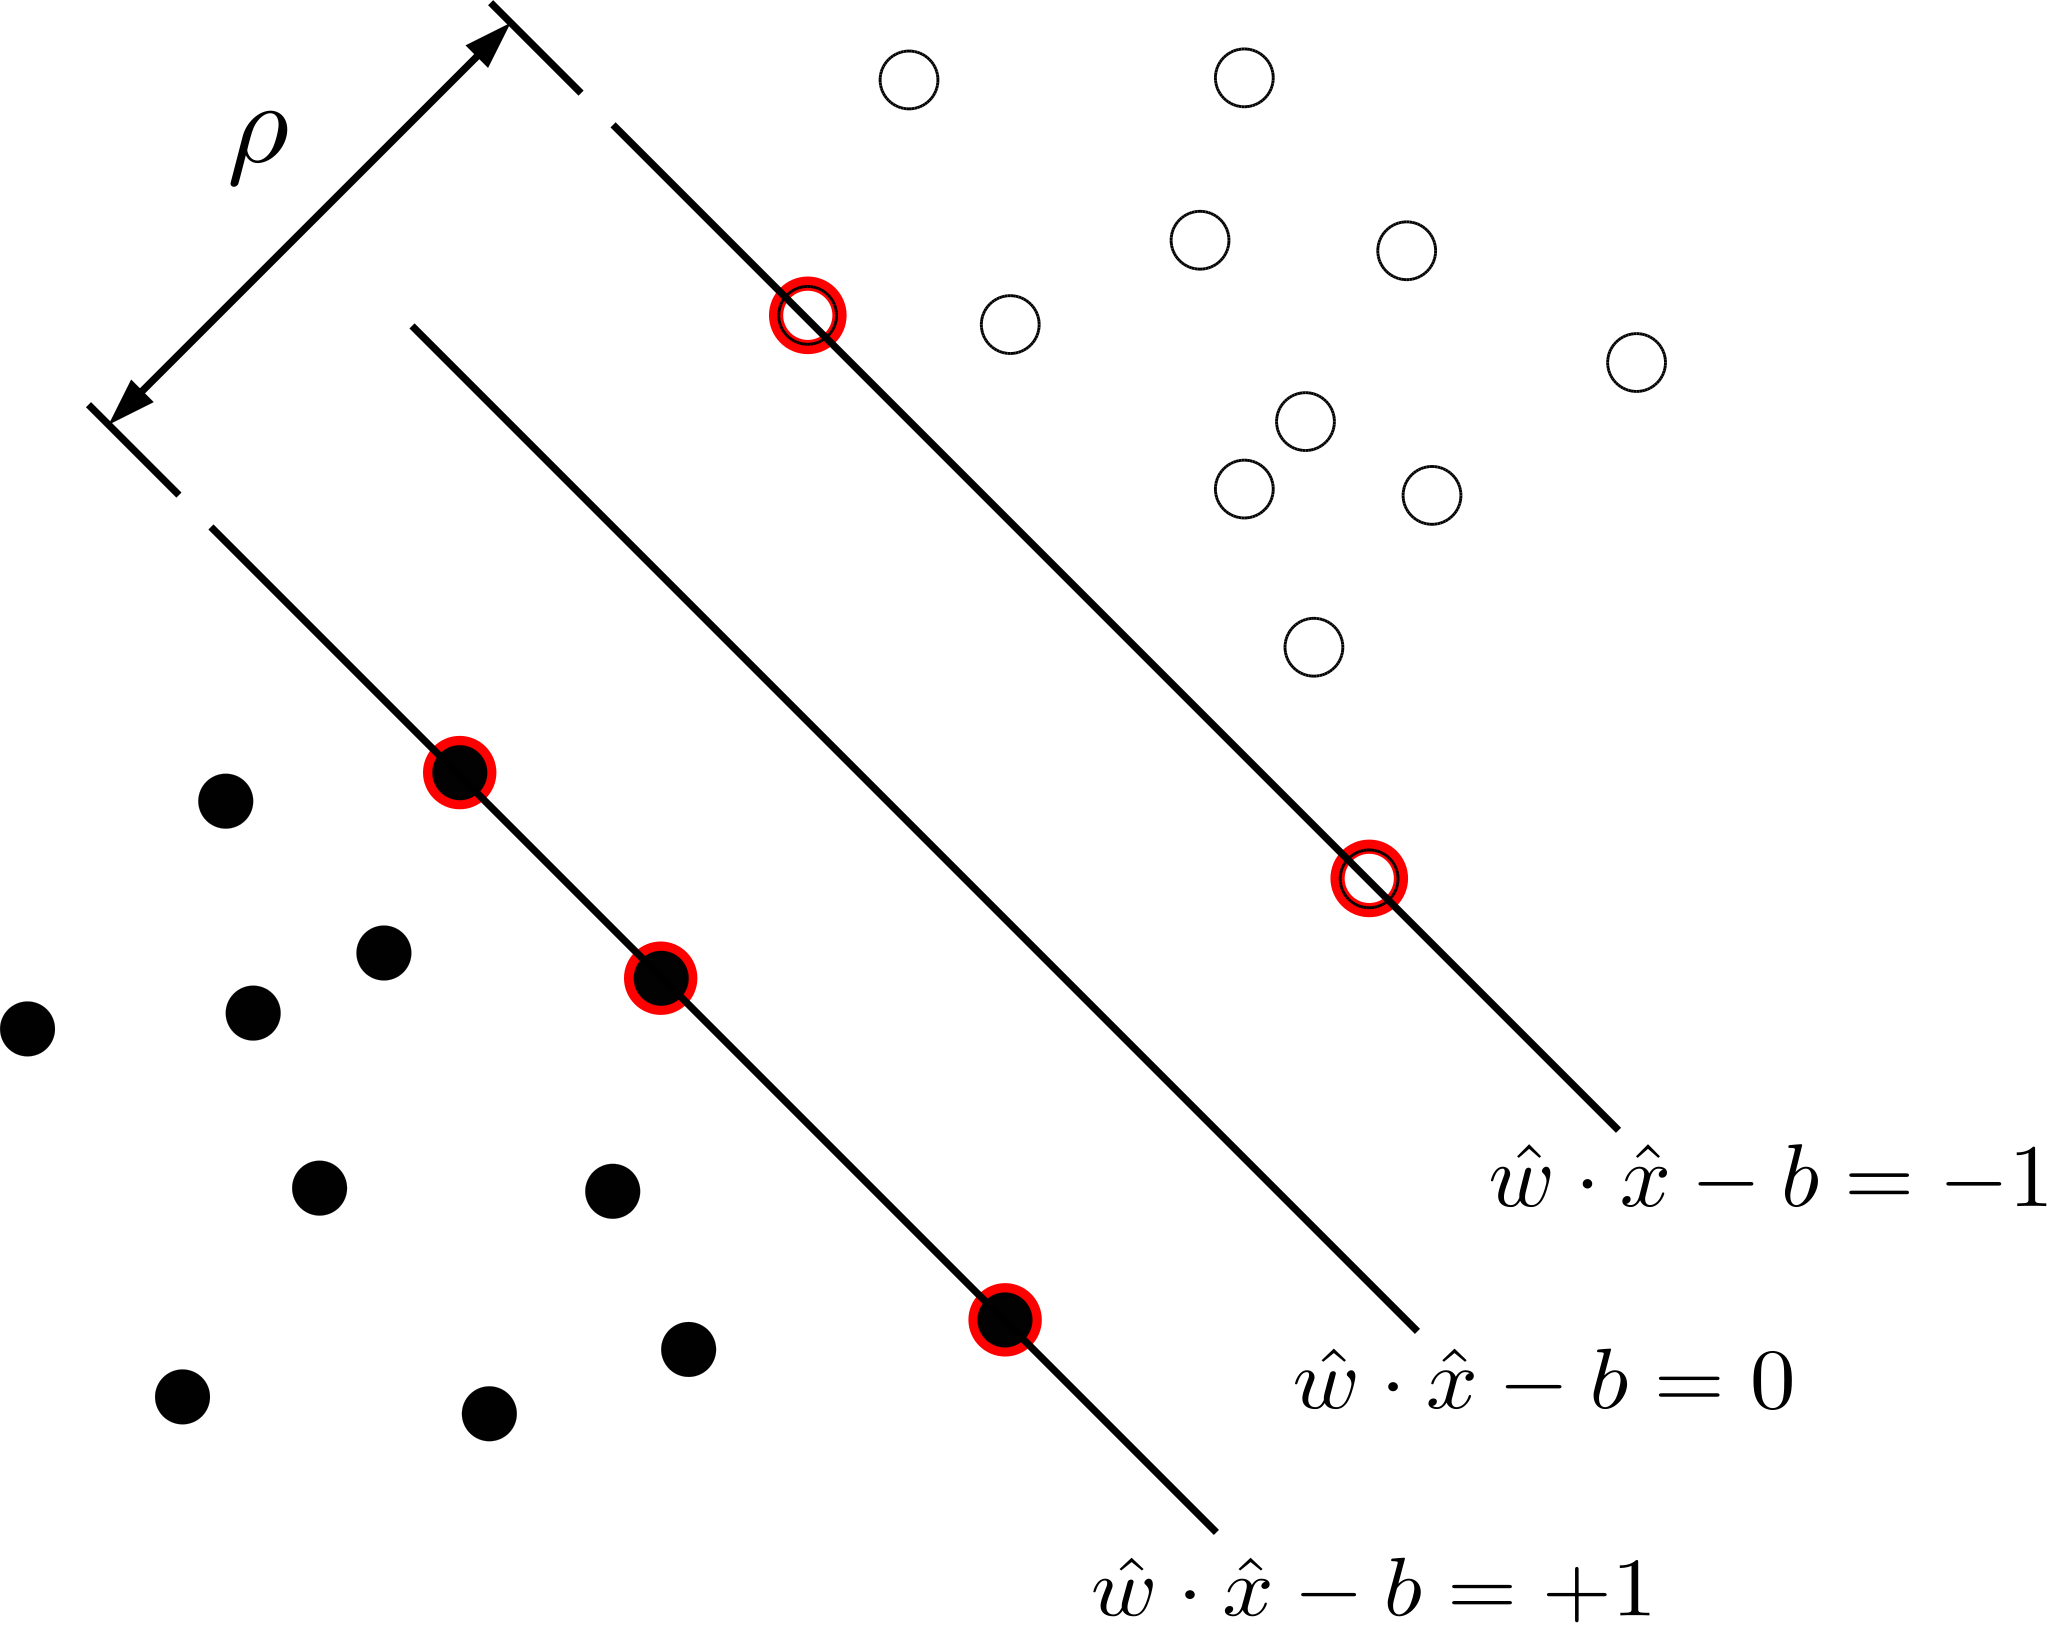
\includegraphics[width=0.65\linewidth]{img/SVM_margins}
	\caption{A hyperplane separating two classes with the maximum margin. The red highlighted points are the support vectors.
	}
	\label{fig:SVM_margins}
\end{figure} 

Formally, suppose that all the data satisfy the constraints

\begin{equation}
\vec{w}\cdot\vec{x}_i + b \geq +1 \text{   for   } y_i = +1,
\end{equation}
\begin{equation}
\vec{w}\cdot\vec{x}_i + b \leq +1 \text{   for   } y_i = -1,
\end{equation}
where $\vec{w}$ is the normal to the hyperplane, $\frac{|b|}{\|\vec{w}\|}$ is the perpendicular distance
from the hyperplane to the origin, and $\|\vec{w}\|$ is the Euclidean norm of $\vec{w}$. These two constraints can be expressed in compact form as:
\begin{equation}
\label{eq:svm_contraint}
y_i( \vec{w}\cdot\vec{x}_i + b)  \geq 1.
\end{equation}
The \textit{canonical hyperplane} is the hyperplane that separates the data and has maximal margin. 
%The training examples that satisfy the \ref{eq:svm_contraint} lie in the \textit{canonical hyperplanes} that satisfy the property
%\begin{equation}
%	\label{eq:canoncal_hyper}
%	\min_{\vec{x}_i \in X} |\vec{w}^T \cdot \vec{x}_i + b | = 1
%\end{equation}
The margin $\rho$ can be computed as the distance
between the two canonical hyperplanes:

\begin{equation}
\label{eq:dinstance_canocical}
\rho = \frac{1 - b}{\|\vec{w}\|} - \frac{- 1 - b}{\|\vec{w}\|} = \frac{2 }{\|\vec{w}\|} 
\end{equation}

Thus, we need to solve an optimisation problem, finding  the hyperplane that maximises the margin and ensures the classes are separable
\begin{equation}
\label{eq:svm_opt_problem}
\min_{\vec{w}_i, b} \frac{1}{2} \|\vec{w}\|^2 \textrm{ subject to } y_i( \vec{w}\cdot\vec{x}_i + b)  \geq 1.
\end{equation}
The problem can be expressed in the Lagrangian formulation:
\begin{equation}
\label{eq:lagrangian_svm_opt_problem}
\mathcal{L}(\vec{w}, b, \lambda) = \frac{1}{2} \|\vec{w}\|^2 + \sum_{i = 1}^{m} \lambda_i(1 -y_i ( \vec{w}\cdot\vec{x}_i + b))
\end{equation}
with Lagrange multipliers $\lambda_i \geq 0$ for each constraint in \ref{eq:svm_opt_problem}. The objective is then to minimize \ref{eq:lagrangian_svm_opt_problem} with respect to $\vec{w}$ and $b$ and simultaneously require that
the derivatives of $\mathcal{L}(\vec{w}, b, \lambda)$ with respect to all the $\lambda$ vanish. The advantage is twofold: the training vectors only appear as a scalar product among the vectors, and the constraints are easier to manage. 

With the formulation presented above, the SVM fails in some situation. In fact, there is no solution if samples can not be separated by a hyperplane. Moreover, although data are linearly separable the SVM may overfit to some outlier compromising system performance. For dealing with this type of problem, has been developed the soft margin SVM \cite{cortes95} which allows data points to lie within the margins. Introducing \textit{slack variables} $\xi_i$ into the constraints and penalize them in objective, the new problem becomes


\begin{equation}
%\begin{eqnarray}
\label{eq:slak_lagrangian_svm_opt_problem}
\min_{\vec{w}_i, b, \vec{\xi}} \frac{1}{2} \|\vec{w}\|^2 +  C\sum_{i = 1}^{m}\xi_i 
%\end{eqnarray}
\end{equation}
\begin{equation}\nonumber
\textrm{ subject to } y_i( \vec{w}\cdot\vec{x}_i + b)  \geq 1 - \xi_i \textrm{ and } \xi_i \geq 0 \textrm{ for } i = 1 \cdots m.
\end{equation}
The cost coefficient C > 0 is a hyper-parameter that specifies the misclassification penalty and is tuned by the user based on the classification task and dataset characteristics.
\paragraph{Non-Linear Support Vector Machines}
A way to solve the problem when data are not linearly separable, is to map the data on to a higher dimensional space and then to use a linear classifier in the higher dimensional space. This methods is referred to as ``the kernel trick '' that exploit the fact that the training data appears as a dot product between vectors in the Lagrangian formulation to from non-linear decision boundaries. Suppose to use a transformation $ \Phi:\vec{x} \to \phi(\vec{x}) $ to map every data sample into higher dimensional space, the dot product becomes $\phi(\vec{x}_i)^{T}\phi(\vec{x}_j)$. By the use of a kernel function 
\begin{equation}
K(\vec{x}_i,\vec{x}_j) = \langle\phi(\vec{x}_i), \phi(\vec{x}_j) \rangle ,
\end{equation}
it
is possible to compute the separating hyperplane without explicitly carrying out
the mapping into feature space. The classifier become:
\begin{equation}
f(\vec{x}) = \mbox{sign}(\sum_i \lambda_i y_i K(\vec{x}_i, \vec{x}_j) + b)
\end{equation}
The most popular kernel functions are:
\begin{itemize}
	\item Linear Kernel: 
	\begin{equation}
	K(\vec{x}_i,\vec{x}_j) = \langle\vec{x}_i, \vec{x}_j \rangle 
	\end{equation}
	
	\item Polynomial Kernel:  	  	 
	\begin{equation}
	K(\vec{x}_i,\vec{x}_j) = (\langle\vec{x}_i, \vec{x}_j \rangle)^d 
	\end{equation}
	\item Sigmoid Kernel: 
	\begin{equation}
	K(\vec{x}_i,\vec{x}_j) = tanh(\gamma\langle\vec{x}_i, \vec{x}_j \rangle -\theta ) 
	\end{equation}
	\item RBF Kernel: 
	\begin{equation}
	K(\vec{x}_i,\vec{x}_j) = \exp(-\frac{\|\vec{x}_i - \vec{x}_j \|}{2\sigma^2})  
	\end{equation}
\end{itemize}

Up to now the SVM algorithm for binary classification has been described. This algorithm can be extended to the multi-class case using the ``one vs all'' technique \cite{bishop06}.


\subsection{One-Class Support Vector Machines}
One-Class SVM (OCSVM) proposed by Sch{\"o}lkopf et al. \cite{scholkopf2000support} is the extension of the support vector machine to the case of unlabeled data that makes them useful for novelty detection problems. In the OCSVM, a new parameter $\nu$ 
that controls the trade-off between maximizing the distance of the hyperplane from the origin and the number of data points contained by the hyperplane has been introduced. To separate the data from the origin, the following quadratic program has to be solved:
\begin{equation}
%\begin{eqnarray}
\label{eq:ocsv_quadratic_problem}
\min_{\vec{w}_i, \vec{\xi}, \rho} \frac{1}{2} \|\vec{w}\|^2 +  \frac{1}{\nu l}\sum_{i = 1}^{m}\xi_i - \rho
%\end{eqnarray}S
\end{equation}
\begin{equation}\nonumber
\textrm{ subject to }\quad ( \vec{w}\cdot \phi(\vec{x}_i))  \geq \rho - \xi_i \textrm{ and } \xi_i \geq 0 \textrm{ for } i = 1 \cdots m.
\end{equation}
In fact, One-Class SVM consists in a discriminant function that takes the value $+1$ in a small region that captures the majority of the data points of a set and $-1$ outside that region \cite{scholkopf2000}. The discriminant function has the following expression:
\begin{equation}\label{eq:svm}
f(\mathbf{x}) = \mathop{\mathrm{sgn}} \left( \sum_{i} \alpha_i \cdot k(\mathbf{x}_i,\mathbf{x}) - \rho\right),
\end{equation}
where $ \vec{x}_i$ denotes the $i$-th support vector. The position of the hyperplane, thus, defines the region that represents normal data points. For each point $\textbf{x}$ that lies outside this region, the function $f( \vec{x})$ takes the value $-1$, whereas for point inside the region, it takes the value $+1$.
The terms $\lambda_i$ can be found by solving the solution to the dual problem:


The terms $\lambda_i$ can be found by solving the solution to the dual problem:
\begin{equation}
\min_{\lambda} \frac{1}{2} \sum_{ij}^{} K(\vec{x_i}, \vec{x_j}) 
\end{equation}
\begin{equation}\nonumber
\textrm{ subject to }\quad 0 \leq \lambda_i \leq \frac{1}{\nu l}\quad \textrm{ and }\quad \sum_{i}^{} \lambda_i = 1,
\end{equation}
where $\lambda_i$ is a Lagrange  multiplier and $l$ is the number of points in the  training dataset.
The term $\nu \in (0,1]$ is an hyperparameter of the algorithm that is determined on a validation set. 

The offset $\rho$ can be obtained from the Karush-Kuhn-Tucker (KKT) condition with the expression \cite{boyd2004convex}:
\begin{equation}
\rho = \sum_j \lambda_i k(\vec{x}_j,\vec{x}_i),
\end{equation}
which is satisfied for any $\lambda_i$ that is not at the upper or lower bound.



\section{Gaussian Mixture Model}
https://pdfs.semanticscholar.org/734b/07b53c23f74a3b004d7fe341ae4fce462fc6.pdf
A Gaussian Mixture Model (GMM) is a parametric probability density function represented as a weighted sum of Gaussian component densities. Generally, GMMs are used as a parametric model of the probability distribution of some features.  To estimate the parameter of GMM the algorithm Expectation-Maximization (EM) algorithm or Maximum A Posteriori (MAP)  are used starting from a well-trained prior model usually named Universal Background Model (UBM).
A Gaussian mixture model is a weighted sum of M component Gaussian densities as given by the equation
\begin{equation}
p(\vec{x, \lambda}) = \sum_{i = 1}^{M} w_i g(\vec{x} |\vec{\mu}_i, \vec{\Sigma}_i)
\end{equation}
where $\vec{x}$ is a D-dimensional features vector, $g (\vec{x} |\vec{\mu}_i), \vec{\Sigma}_i)$ are the components of the mixture and $w_i$ are the weight of each component. Each component of the mixture is a D-variate Gaussian density function expressed as
\begin{equation}
a
\end{equation}
\section{K-Nearest Neighbor}
\section{Deep Neural Network}
\subsection{Convolutional Neural Network}
\subsection{Autoencoder}
%\subsection{Siamese Neural Network}




\graphicspath{{3_datasets/}}
\chapter{Dataset}
\label{ch:dataset}
%poichè non erano presnti dataset adui suabili, ce ne siamo fatti uno noi. Poi per ogni metodo verranno esplicitati i dati usati.

The importance of using public data sets for algorithm evaluation is very important. Only in this way can a direct comparison be made between the different approaches to determine which of these is actually the best. There are publicly available datasets for the fall detection task, the majority of them are all related to wearable or vision sensors and often include both types \cite{spinsantefalldata, kwolek2014human, charfi2013optimized, s140610691, s17071513}. Since in this work, we face the problem fall detection from an audio perspective, only one dataset containing audio recording has been found \cite{cirdodataset}. However, the audio files available in the dataset are suitable for speech recognition related works rather than sound event detection. In fact, only the utterance of short sentences or interjections of the actors involved during the human falls recordings have been annotated. As in this work, several data-driven approaches for pattern recognition produced by the sound generated by the human fall are presented, the dataset \cite{cirdodataset} result useless. Given the lack of available audio data sets, we have created a suitable audio dataset in order to assess the proposed approaches. This choice was also forced by the fact that in these works an innovative acoustic sensor was explicitly developed for the fall detection and described in \secref{sec:sensor} has been used.
In this chapter, the instrumentation, the procedure for recording the audio corpus and its composition are described.

\section{The floor acoustic sensor}
\label{sec:sensor}

\begin{figure}[t]
	\centering
	\includegraphics[width=0.8\textwidth]{img/AcousticSensor.pdf}
	\caption{The floor acoustic sensor: conceptual scheme. \mbox{1 - The} outer container. \mbox{2 - The} inner container. \mbox{3 - The} microphone slot. \mbox{4 - The} membrane touching the floor.}
	\label{fig:case}
\end{figure}
The floor acoustic sensor (FAS) is composed of a resonant enclosure and a microphone located inside it (\figref{fig:case}) \cite{Olivetti15}. At the bottom of  the enclosure, a membrane  is in direct contact with the floor and guarantees the acoustic coupling with the surface. The inner container accommodates the microphone and is where the acoustic resonance phenomenon takes place. It can be covered by a layer of acoustic isolation material and it is enclosed by the outer container that further reduces the intensity of the acoustic waves that propagate through air. The enclosure has been manufactured in Polylactic Acid with a 3D printer, its diameter is 16.5\,cm and its height 5.5\,cm.

%The acoustic sensor used in the sound database acquisition (as described in \secref{Experiments}) is depicted in \figref{fig:meringa}. The dimensions of the acoustic sensor are the following: 16.5\,cm of diameter and 5.5\,cm of height. The material used for the sensor case, developed through the 3D printing technology, is Polylactic Acid. %No acoustic isolation material has been inserted into the space between the inner and outer container.

Regarding the microphone, an AKG C 400 BL\footnote{http://www.akg.com/pro/p/c400-bl} has been inserted in the enclosure. The outer case of the microphone has been removed to extract the capsule that has then been inserted in the sensor enclosure. The AKG C 400 BL is characterized by an hypercardiod directivity pattern, thus it has been oriented so that the maximum gain is towards floor.

\begin{figure}[t]
	\centering
	\includegraphics[width=0.8\columnwidth]{img/FAS_front_little.jpg}
	\caption{A picture of the floor acoustic sensor used during the recordings.} \label{fig:meringa}
\end{figure}

\section{The fall events dataset: A3Fall}
\label{sec:dataset}
The performance of the floor acoustic sensor has been evaluated on a corpus of audio events corresponding to falls of several objects recorded in different conditions\footnote{The dataset is available at the following URL: \url{http://www.a3lab.dii.univpm.it/research/fasdataset}}. The dataset has been specifically created by the authors and it will be presented in this section.

\subsection{The recording setup}
Fall events have been recorded in 3 different rooms with the following characteristics:
\begin{itemize}
	\item The first, is a rectangular room, hereafter named R0, measuring about 7\,m\,$\times$\,2\,m (\figref{fig:room}). The room is particularly suitable for the propagation of acoustic waves through the floor since it is obtained from a cantilever beam. In addition, the considerable distance of the supporting pillars facilitates the transmission of a fall vibrations through the floor.
	\item the second location for the recording was the university auditorium room (R1) in which the flooring is composed of fitted carpet. This makes it particularly suitable for evaluating system performance on surfaces with acoustical behavior that can mitigate the impact sound transmitted through the floor and in the air; all the recordings were performed near the auditorium stage in an area of 8$\times$3\,m.
	\item a recording studio (R2) was selected as the third location for its particular characteristics. Here, it was possible to make the acquisitions by placing the sensors in the live room while the audio events were performed in the control room. In particular, the sensors were positioned immediately behind the soundproof wall with the window overlooking the live room. The size of the live room is 5$\times$7\,m, while the size of the control room is 3$\times$8\,m.
\end{itemize}

  The recording equipment comprises the floor sensor, a linear array of three aerial microphones (the same AKG 400 BL included in the floor sensor) and a Presonus AudioBox 44VSL sound card connected to a laptop. The microphones of the array are separated by 4\,cm and positioned on a table 80\,cm high. Signals were sampled at 44.1\,kHz with a resolution of 32\,bits. Levels were calibrated to assure the maximum dynamic range at the smallest distance.

\subsection{Description}
In \tableref{tab:numDataset} the composition of the dataset is summarized.
For the R0, the dataset comprises recordings of fall events related to everyday objects and to a human mimicking doll. The objects were chosen according to the recent literature on the topic \cite{alwan2006smart} and are the following: a ball, a metal basket, a book, a metal fork, a plastic chair, and a bag (\figref{fig:objects}). Objects have been dropped at four distances from the sensors, i.e., 1\,m, 2\,m, 4\,m, and 6\,m, and with various angles in order to reproduce realistically different fall patterns. With the exception of the chair and the basket, which have been overturned from their natural position, half of the falls has been performed at a height of 0.5\,m and the other half at 1\,m. For each object and for each distance, 16 fall events have been performed for a total of 64 events per object. Instead, the chair has been overturned 8 times for each side of fall (back, front, side) and for each distance, thus obtaining a total of 96 events.

\begin{table}[t]
	\caption{Composition of the A3Fall-v2.0 dataset.}
	\label{tab:numDataset}
	\begin{center}
		\begin{tabular}[t]{c|ccc}
			
			\hline
			\textbf{Class} & \textbf{R0} & \textbf{R1} & \textbf{R2} \\ %\cline{2-5} 
			%& \hspace{8pt}Clean\hspace{8pt}  & \hspace{6pt}Clean\hspace{6pt}   \\ 
			\hline
			&\multicolumn{3}{c}{Nr. of occurrences}\\
			Basket      			& 64    &   40 	&   40    	\\
			Fork        			& 64    &   40 	&   40     	\\
			Ball       				& 64    &   40	&   40    	\\
			Book        			& 64    &   40	&   40    	\\
			Bag         			& 64    &   30 	&   40    	\\
			Chair       			& 96    &   40 	&   40    	\\
			Table       			& 0   	&   40 	&   40    	\\
			Guitar Slide       		& 0   	&   40 	&   40    	\\
			Nipper       			& 0    	&   40 	&   40    	\\
			Keys       				& 0    	&   40 	&   40    	\\
			Hook       				& 0    	&   40 	&   40    	\\
			Coat Hook       		& 0    	&   40 	&   40    	\\
			$\,$ Manikin Doll $\,$ 	& 44    &   0 	&   0    	\\
			$\,$ Human Fall $\,$ 	& 0    	&   40 	&   40    	\\
			\hline
			&\multicolumn{3}{c}{Total length (s)}\\			
			%			Human Activity  		& 1135  &   3050&   580   	\\
			%			Music					& 1395  &	4330&   3345  	\\
			%			Television				& 0   	&	1675&   1625  	\\
			Background  			& 2530  &   9055&   5550   	\\
			\hline
		\end{tabular}
	\end{center}
\end{table}

\begin{figure}[t]
	\centering
	\includegraphics[width=0.4\textwidth]{img/oggetti_cadute3.jpeg}
	\caption{Objects employed for creating the fall events dataset.}\label{fig:objects}
\end{figure}

Human falls have been simulated by employing the ``Rescue Randy'' doll\footnote{http://www.simulaids.com/1475.htm}, a professional equipment employed in water rescues. It weights 75\,kg, it is 1.85\,m high, and it is equipped with articulated joints. The doll is made of vinyl and its weight is distributed according to the human weight distribution chart. The doll has been dropped from upright position and from a chair, both forward and backward, for a total of 44 events (\figref{fig:randy}). Differently from the everyday objects, the distribution of the fall events with the distance is not uniform: 10 events have been performed from 2\,m, 18 from 4\,m (7 of which from the chair), and 16 from 6\,m (6 of which from the chair).

Moreover, several backgrounds sounds has been added to the dataset. 
Normal activities sounds have been recorded while persons were performing common actions, such as walking, talking, and dragging chairs. Three musical tracks have been played from a loudspeaker and acquired back with the FAS. The first track contained classical music\footnote{W. A. Mozart, ``Piano trio in C major''}, while the second\footnote{Led Zeppelin, ``Dazed and confused''} and the third\footnote{Led Zeppelin, ``When the levee breaks''} rock music. Musical tracks and normal activities sounds have been divided in segments whose lengths have mean and standard deviation estimated from instances of fall events. In addition, they have been employed alone and to create noisy versions of human and object falls occurrences in order to assess the algorithm in presence of interferences. 

In R2 and R1 other every-days objects,in addition to those used in R0, have been recorded for a total of 12 different object fall classes and 1420 instances. While the manikin doll has been used only in R0, in R1 and R2 a total 80 human falls have been performed by 4 people. These falls were performed in different ways: forward, backward and on the side, trying to use the arms to cushion the fall and without any protections. As in R0, also in R2 and R2 all events were performed from 1, 2, 4 and 6 m away from the FAS.

\begin{figure}[t]
	\centering
	\begin{subfigure}[b]{0.40\textwidth}
		\includegraphics[width=\textwidth]{img/impalcatura.jpg}
		\caption{Fall from upright position.}\label{fig:randy_upright}
	\end{subfigure}
	\begin{subfigure}[b]{0.40\textwidth}
		\includegraphics[width=\textwidth]{img/rndy_caduta_sedia.jpg}
		\caption{Fall from the chair.}\label{fig:randy_chair}
	\end{subfigure}
	\caption{Falls of the ``Rescue Randy'' doll from upright position (a) and from the chair (b).}\label{fig:randy}
\end{figure}

\begin{figure}[t]
	\centering
	\includegraphics[width=\columnwidth]{img/room_experiments.pdf}
	\caption{The recording room: the letters A, B, C and D indicate the positions of fall events.}
	\label{fig:room}
\end{figure}

As shown in \tableref{tab:numDataset} background noises have been recorded also in R1 and R2 rooms rooms, which include: human activities noise as, i.e., footsteps, human and phone conversation, dragging objects and so on; classic, rock and pop music played from loudspeakers; TV shows like newscast and satiric.

Since the data relating to rooms R1 and R2 have been collected at different times to those of room R0, in the following chapters, for each proposed approach, it will be specified which subset of the total dataset has been used as well as the usage of the noisy version of falls events.


\subsection{Signal analysis}\label{ssec:sig_analysis}
The signal related to the same fall event acquired with the floor sensor and with the aerial microphone exhibits different spectral characteristics. In this section and in depth analysis of the audio signals acquired in the R0 room is presented. \figref{fig:spectrograms} shows the spectrograms of a doll fall acquired with the floor sensor (above) and with the aerial microphone (below) in the clean acoustic condition. Observing the figures, it can be noticed that the aerial microphone is more sensitive to high frequencies, in particular to the ones above 1.5\,kHz. On the contrary, the majority of the energy of the signal acquired with the floor sensor concentrates below 1\,kHz. 

This is even more evident by plotting the values of the mel coefficients (\figref{fig:mel}): the first and second mel channels of the FAS, corresponding to the frequency bands 0--128.10\,Hz and 61.30-200.60\,Hz, are higher respect to the aerial microphone. Channels 3 to 7, respectively corresponding to bands 128.10--279.50\,Hz and 458.70--670.70\,Hz, are almost equivalent, while from channel 8 (560.30--790.80\,Hz) to 29 (6654.60--8000.00\,kHz) the aerial microphone mels are greater.

\begin{figure}[t]
	\centering
	\begin{subfigure}[b]{0.8\textwidth}
		\includegraphics[width=\textwidth]{img/spettro_fas}
		\caption{Spectrogram of the signal acquired with the floor sensor.}
		\label{fig:spec_fas}
	\end{subfigure}
	\begin{subfigure}[b]{0.8\textwidth}
		\includegraphics[width=\textwidth]{img/spettro_mic}
		\caption{Spectrogram of the signal acquired with the aerial microphone.}
		\label{fig:spec_aer}
	\end{subfigure}
	
	\caption{Frequency content of the same fall event (file ``rndy\_d2st\_bar\_0.wav'') acquired with the FAS (a) and with the aerial microphone (b).}\label{fig:spectrograms}
\end{figure}

\begin{figure}[t]
	\centering
	\includegraphics[width=0.75\textwidth]{img/mel_dB}
	\caption{Average value of the mel channels.} \label{fig:mel}
\end{figure}

\begin{figure}[t]
	\centering
	\includegraphics[width=0.75\textwidth]{img/SNR_mel_channel}
	\caption{Average value of the SNR for each mel channel.} \label{fig:noisymel}
\end{figure}

The analysis of noisy signals highlights the different behaviour of the floor sensor respect to the aerial microphone in presence of external interferences. 
In fact, taking into account the backgrounds tracks as interferences, the floor sensor has a global signal-to-noise ratio (SNR) equal to 20.94\,dB and a segmental SNR equal to 7.28\,dB. The global SNR of the central aerial microphone is 8.92\,dB and the segmental SNR is -1.47\,dB. The values of the aerial microphone SNRs are thus considerably lower than the ones of the floor sensor.%: this highlights the superiority of the FAS respect to the aerial microphone in reducing sounds propagating through the air and not related to fall events.
The global SNR of the floor sensor noisy dataset is 13.66\,dB higher than the one of the aerial microphone, highlighting the superior ability of the former to isolate fall signals from external interferences. However, it is worth investigating how the SNR distributes over the frequency range of the acquired signals in order to have a better insight of the physical phenomenon. \figref{fig:noisymel} shows the SNR calculated for each mel channel and averaged across the noisy datasets. It can be noticed that the SNR of the floor sensor exceeds the one of the aerial microphone for channels below the fourth. Then, the opposite occurs and the SNR of the aerial microphone assumes greater values. The ``valley'' in the curves are due to the pitch of the music signal.




\graphicspath{{4_Supervised_approaches/}}
\chapter{Supervised Approach}
qua vengono presentati sia il metodo multilabel classifier GMM-UBM SVM (ESWN) che 
il binary  GMM-UBM SVM (WIRN2016)



\section{Support-Vector Machine based algorithm for evens fall classification}
\label{sec:algorithm_svm_multiclass}
The fall detection task consists in recognize which object produced the pattern of a signal and it mainly consists of two subtasks: the location of the time boundaries of the fall event and the classification of that event. In this section, we concentrate on the second subtask, since the main objective is determining the performance of the acoustic sensor as compared to common aerial microphones. The entire falls detection activity will be addressed in the works presented below.

The fall classification algorithm is composed of a feature extraction stage and a classification stage. The first extracts MFCCs from the input audio signal, while the second classifies the audio event by means of Gaussian means supervectors and SVM. Following is a detailed description of the two stages.

\subsection{Feature extraction}\label{ssec:fx}
Despite MFCCs were originally developed for speech and speaker recognition tasks, they have been successfully applied also for acoustic event classification \cite{Temko2009} and fall detection \cite{zigel2009method}.

\begin{figure}[b]
	\centering
	\includegraphics[width=0.75\columnwidth]{img/mfcc_bn.pdf}
	\caption{The MFCC feature extraction pipeline.} \label{fig:mfcc}
\end{figure}

The block-scheme of the MFCC feature extraction pipeline is shown in \figref{fig:mfcc}. The first processing step is the pre-emphasis of the input signal, which consists in applying a filter whose transfer function is:
\begin{equation}
G(z) = 1 - \alpha z^{-1}.
\end{equation}
Usually $0.9<\alpha\leq1.0$ and here it has been set to 0.97. The objective of pre-emphasis is to remove the DC components and to raise the high-frequency part of the spectrum.

The signal is then segmented in frames 16\,ms long overlapped by 8\,ms and multiplied with a Hamming window. For each frame, the Discrete Fourier Transform (DFT) is calculated and filtered with a filterbank composed of 29 triangular filters uniformly spaced on the mel scale. 

Denoting with $S(i)$ the DFT of a frame and $i$ the frequency bin, the output of the ``Mel Filterbank \& Frequency Integration'' block in \figref{fig:mfcc} is
\begin{equation}
mel(k) = \sum_{i=ini(k)}^{end(k)}|S(i)|^2 W_k(i), \qquad k=1,2,\ldots,N
\end{equation}
where $mel(k)$ is the energy of the $k$-th subband, $W_k(i)$ is the frequency response of the $k$-th filter, $ini(k)$ and $end(k)$ are starting and ending frequency indices of that filter and $N$ is the number of filters in the bank, which in this case is 29. The terms $mel(k)$ are often named ``mel coefficients''.

The final steps for the calculation of the $j$-th MFCC $c(j)$ is the logarithm and the Discrete Cosine Transform (DCT):
\begin{equation}
\begin{aligned}
c(j) = \sum_{k=1}^{N}\log \left[ H(k)\right] \cos\left[\frac{\pi j}{N}(k-0.5)\right], \quad j=0,1,\ldots,M-1\leq N
\end{aligned}
\end{equation}
The set $\{c(0),c(1),\ldots,c(M-1)\}$ forms the static coefficients elements of the feature vector. Here $M$ has been set to 13. The final feature vector is composed of 39 coefficients, i.e., the 13 static coefficients plus their first and second derivatives. %  MFCCs have been extracted with the HCopy tool of the Hidden Markov Model Toolkit \cite{Young2006}.

%Cepstral Mean Normalization (CMN) is then applied to MFCCs to increase the robustness against channel distortions. CMN consists in subtracting the mean of each cepstral coefficients calculated over the entire event:
%\begin{equation}
%c'_t(n) = c_t(n) - \frac{1}{T}\sum_{l=0}^{T-1}c_l(n), \qquad t=0,1,\ldots,T-1
%\end{equation}
%where $t$ denotes the time frame index and $T$ is the event length in frames.

\subsection{Classification stage}
\label{sec:svm_multi_classification}
The approach proposed in this section is based on a One-Class Support Vector Machine (OCSVM) \cite{scholkopf2000}. The general idea is that a human fall produces a sound considerably different from the ones commonly occurring in a home (e.g., voices, sounds from electronic devices, footsteps, etc.). The OCSVM is trained on a large set of ``normal'' sounds to detect acoustic events that deviate from normality. However, it is expected that certain acoustic events are as abnormal as a human fall (e.g., the fall of book, a chair, etc.), thus they could raise false alarms. 



The classification stage employs Gaussian Mean Supervectors (GMS) and a Support Vector Machine classifier as in speaker recognition systems \cite{kinnunen10}. The algorithms consists in modelling the entire acoustic space with a Universal Background Model (UBM) represented by mixture of gaussians (Gaussian Mixture Model, GMM). The GMM is trained using the Expectation Maximization (EM) algorithm \cite{bilmes1998gentle} on a large corpus of acoustic events. Then, for each acoustic event class in the training corpus a GMS is calculated by adapting the UBM with the Maximum A Posteriori (MAP) algorithm \cite{reynolds10} and concatenating the adapted GMM mean values. The block diagram of the approach is shown in \figref{fig:gms}. The final step of the training phase is the estimation of the SVM parameters. In this work, an SVM with a radial basis function has been used. The complete diagram of the training phase is shown in \figref{fig:training-scheme}.

Classification is performed by extracting the supervector from an input audio signal as in the training phase, and then determining the acoustic event class evaluating the SVM discriminant function (\figref{fig:scheme-classify-color}). Since the number of classes is greater than two and SVMs are binary classifiers, the ``one versus all''  technique has been adopted \cite{bishop06}. LIBSVM \cite{chang11} has been employed both in the training and testing phases of the SVM.

\begin{figure}[t]
	\centering
	\includegraphics[width=0.75\columnwidth]{img/gms_bn.pdf}
	\caption{Block scheme for extracting a gaussian mean supervector from MFCCs and a trained UBM.} \label{fig:gms}
\end{figure}

\begin{figure}[t]
	\centering
	\includegraphics[width=0.3334\columnwidth]{img/training_scheme.pdf}
	\caption{Block scheme for training the UBM and SVM models.}
	\label{fig:training-scheme}
\end{figure}

\begin{figure}[t]
	\centering
	
\includegraphics[width=0.333\columnwidth]{img/scheme_classify_bn.pdf}
	\caption{Block-scheme of the fall classification phase.}
	\label{fig:scheme-classify-color}
\end{figure}

\section{Experiments}\label{sec:experiments}

This section firstly presents presents which portion of the dataset described in \secref{sec:dataset} has been used in this work, then the classification performance of the algorithm. 

\subsection{Dataset}
\label{sec:dataset_svm_multiclass}
All the experiments have been conducted data related to R0 room only. In particular, in order to compare the performance of the FAS with a standard aerial microphone, not all data concerning all the aerial microphones array have been used but only the one of the microphone closest to the wall (see \figref{fig:room}). Moreover, signals have been downsampled to 16\,kHz and the resolution has been reduced to 16\,bit. In order to obtain a balanced dataset, for each object and
for each distance, 11 fall events have been randomly picked for a total of 44 events per
object, while all the 44 simulated human fall with the manikin has been selected. In addition, the three musical track recored in the R0 room have been employed to create a noisy version of
the dataset by digitally adding a random segment of the recorded musical tracks
to the ``clean'' datasets as was done for the analysis of the signals in \secref{ssec:sig_analysis}. In particular, the analysis presented in \secref{ssec:sig_analysis} suggested the authors that the standard MFCC extraction pipeline can be modified in order to better exploit the properties the floor acoustic sensor. In particular, the analysis led to the following considerations:
\begin{itemize}
	\item The pre-emphasis filter is an inheritance of automatic speech recognition systems, where the input signal is the human voice. Since the effect of the filter is to enhance the high frequency components of the signal and the floor sensor is more sensitive to low frequencies, removing the pre-emphasis could improve the classification performance.
	\item The majority of the energy of the signals acquired with the floor acoustic sensor is concentrated at frequencies below 1.5\,kHz. This suggest that introducing a low-pass filter that removes low SNR frequencies may improve the classification performance.
\end{itemize}
In \tableref{tab:eswa_dataset} the data used for this approach are summarized.
\begin{table}[t]
	\caption{Data related to R0 room used in this work.}
	\label{tab:eswa_dataset}
	\begin{center}
		\begin{tabular}[t]{c|c}
			
			\hline
			\textbf{Classes}  & \textbf{Nr. of occurrences} \\ %\cline{2-5} 
			%& \hspace{8pt}Clean\hspace{8pt}  & \hspace{6pt}Clean\hspace{6pt}   \\ 
			\hline
			
			Basket      			&   44    	\\
			Fork        			&   44     	\\
			Ball       				&   44    	\\
			Book        			&   44    	\\
			Bag         			&   44    	\\
			Chair       			&   44    	\\
			$\,$ Manikin Doll $\,$ 	&   44    	\\
			\hline
			\textbf{Backgrounds} & \textbf{Total length (s)}\\			
			%			Human Activity  		& 1135  &   3050&   580   	\\
			%			Music					& 1395  &	4330&   3345  	\\
			%			Television				& 0   	&	1675&   1625  	\\
			Classic Music  			&   882   	\\
			Rock Music  			&   616   	\\
			\hline
		\end{tabular}
	\end{center}
\end{table}

\subsection{Experimental setup}
The MFCC extraction pipeline has been firstly parametrised as described in \secref{ssec:fx}, then, based on the study presented in the previous section, two additional pipelines have been tested:
\begin{itemize}
	\item no pre-emphasis (NOPRE): the pre-emphasis stage has been removed from the feature extraction pipeline;
	\item no pre-emphasis plus low-pass filtering (NOPRELP): the pre-emphasis stage has been removed and the maximum frequency of the mel filterbank has been set to 4\,kHz.
\end{itemize}
The standard MFCC extraction pipeline described in \secref{ssec:fx} will be denoted with ``STD'' in the results.

Regarding the UBM, it has been trained until convergence with the EM algorithm setting the threshold value to $10^{-3}$. The same value has been employed in the MAP adaptation algorithm, but the maximum number of iterations was set to 5.

Due to the limited amount of data, the experiments have been conducted with the leave-one-label-out method: fall events recorded at all distances but one were employed for training and validation, while the remaining for testing. The validation phase consisted in searching for the number of components of the UBM and for the SVM hyperparameters which yielded the best results. In particular, the number of components of the UBM assumed the values $\{ 1,2,\ldots,64 \}$, while the SVM hyperparameters $C$ and $\gamma$ the values $\{ 2^{-5},2^{-3},\ldots,2^{15} \}$ and $\{ 2^{-15},2^{-13},\ldots,2^{3} \}$ respectively. 

The performance was evaluated both on clean data and on data corrupted with the music interference. In particular, the system was evaluated in matched condition, where the acoustic scenario of the training, validation and test data is the same, in mismatched condition, where training data is clean and testing data is corrupted with music, and in multi-condition, where training data and testing data contain both clean signals and corrupted signals. In the latter case, the training, validation and test sets have been divided so that they contain 1/3 of clean data and 2/3 of noisy data.

The performance has been evaluated in terms of precision ($P$), recall ($R$) and F$_1$-Measure ($F$) per class and the values have then been averaged. The metrics definitions for class $i$ is:
\begin{align}
P_i &=  \frac{C(i,i) }{\sum_j C(j,i)}, \\
R_i &=  \frac{C(i,i) }{\sum_j C(i,j)}, \\
F_{i} &= \frac{2P_iR_i}{P_i+R_i},
\end{align}
where $C=[C(i,j)]$ is the confusion matrix.

%\begin{table}[t]
%\centering
%\caption{Number of fall events employed for training, validation and testing. \textbf{@Diego: completare.}}\label{tbl:tvtsplit}
%\begin{footnotesize}
%\begin{tabular}{r | c c c c c c c | c}
%\hline						 
%						 & \textbf{Volleyball} & \textbf{Basket} & \textbf{Book} & \textbf{Fork} & \textbf{Chair} & \textbf{Bag} & \textbf{Doll} & \textbf{Total} \\						 
%\hline
%\textbf{Training}     & 32 & 32 & 32 & 32 & 48 & 32 & -- &    --      \\
%\textbf{Validation}   & 16 & 16 & 16 & 16 & 24 & 16 & --  &    --         \\
%\textbf{Testing}      & 16 & 16 & 16 & 16 & 24 & 16 & -- &     --        \\
%\hline
%\end{tabular}
%\end{footnotesize}
%\end{table}

%The best performance was obtained by using an UBM with 16 mixtures, $C=\{2,2,2^{-1},2\}$ and $\gamma=\{2^{-9},2^{-9},2^{-7},2^{-7} \}$. The values of $C$ and $\gamma$ are four since they are specific for each test fold.

\subsection{Results in matched condition}
\figref{fig:results_match} shows the results obtained in matched condition. As shown in the figure, the FAS exceeds the F$_1$-Measure of the aerial microphone both with clean and noisy signals regardless the feature setup employed. In particular, in clean conditions the aerial microphone achieves the highest F$_1$-Measure with standard MFCCs, while the FAS with the NOPRELP ones, which results in 6.50\% absolute improvement. In noisy conditions, the aerial microphones best performance is again achieved with STD features, while the FAS one is achieved with the NOPRE features, with the NOPRELP setup performing almost the same. The absolute improvement of the FAS respect to the aerial microphone is 5.36\%.

\begin{figure}[t]
	\centering
	\begin{subfigure}[b]{0.6\textwidth}
		\includegraphics[width=\textwidth]{img/pgfsources/16_matched_clean/16_matched_CLEAN.pdf}
		\caption{}\label{fig:results_match_clean}
	\end{subfigure}
	\begin{subfigure}[b]{0.6\textwidth}
		\includegraphics[width=\textwidth]{img/pgfsources/16_matched_noisy/16_matched_NOISY.pdf}
		\caption{}\label{fig:results_match_noisy}
	\end{subfigure}
	\caption{Fall classification performance in matched condition with clean (a) and noisy signals (b).} \label{fig:results_match}
\end{figure}

Focusing on the FAS performance with the various feature extraction pipelines, the highest F$_1$-Measure is obtained by removing the pre-emphasis and low-pass filtering the signals (NOPRELP) in clean conditions. Notice, however, the standard pipeline performs almost the same, thus in this condition the influence is minimal. The sole removal of the pre-emphasis, on the other hand, is detrimental for the classification performance. The opposite occurs in noisy condition, where the removal of the pre-emphasis improves the results by 3.99\%. Low-pass filtering, on the other hand, does not give further improvements. Overall, the feature pipeline that gives the highest F$_1$-Measure is the NOPRELP, as argued in \secref{ssec:sig_analysis}.

Further insights on the results are given by the confusion matrices of the aerial microphone (\tableref{tbl:cm_mic_clean_matched_np}) and of the FAS (\tableref{tbl:cm_fas_clean_matched_npre4k}) for the feature pipeline giving the highest F$_1$-Measure. With the only exception of the basket falls, the FAS is able to achieve superior performance for all the objects in the dataset. In particular, the doll F$_1$-Measure improves by 9.89\% respect to the aerial microphone. The object exhibiting the lowest performance regardless the sensor is the book: this can denote a limit in the algorithm suggesting that further improvements could be obtained by properly modifying the features or the classifier.

\begin{table}[t]
	\caption{Aerial microphone confusion matrix related to the STD configuration in clean condition. The average precision is 91.48\%, the average recall 91.23\%, and the average F$_1$-Measure 91.04\%.}
	\label{tbl:cm_mic_clean_matched_np}
	\centering
	\footnotesize
	\begin{tabular} {r  *{7}{E} | c|}
		\hhline{~*{8}-}
		\multicolumn{1}{c}{} & \multicolumn{1}{|c}{\textbf{Doll}} & \multicolumn{1}{c}{\textbf{Bag}} & \multicolumn{1}{c}{\textbf{Ball}} & \multicolumn{1}{c}{\textbf{Basket}} & \multicolumn{1}{c}{\textbf{Book}} & \multicolumn{1}{c}{\textbf{Chair}} & \multicolumn{1}{c|}{\textbf{Fork}} 
		& \multicolumn{1}{c|}{\textbf{F$_1$}}\\
		\hhline{*{9}{-|}}
		\multicolumn{1}{|r|}{~\textbf{Doll}} & 93.18 & 0 & 0 & 0 & 2.27 & 4.55 & 0 & 90.11 \\ 
		\multicolumn{1}{|r|}{~\textbf{Bag}} & 0 & 86.36 & 0 & 0 & 13.64 & 0 & 0 & 82.61 \\
		\multicolumn{1}{|r|}{~\textbf{Ball}} & 0 & 0 & 100.00 & 0 & 0 & 0 & 0 & 100.00 \\  
		\multicolumn{1}{|r|}{~\textbf{Basket}} & 2.27 & 0 & 0 & 97.73 & 0 & 0 & 0 & 98.85 \\ %\hline
		\multicolumn{1}{|r|}{~\textbf{Book}} & 0 & 22.73 & 0 & 0 & 77.27 & 0 & 0 & 78.16\\ %hline
		\multicolumn{1}{|r|}{~\textbf{Chair}} & 11.36 & 0 & 0 & 0 & 4.55 & 84.09 & 0 & 89.16 \\ %\hline
		\multicolumn{1}{|r|}{~\textbf{Fork}} & 0 & 0 & 0 & 0 & 0 & 0 & 100 & 100.00\\ \hhline{*{9}{-}}
		\multicolumn{1}{|r|}{~\textbf{Precision}} & \multicolumn{1}{c}{87.27} & \multicolumn{1}{c}{79.17} & \multicolumn{1}{c}{100.00} & \multicolumn{1}{c}{100.00} & \multicolumn{1}{c}{79.07} & \multicolumn{1}{c}{94.87} & \multicolumn{1}{c|}{100.00} & \multicolumn{1}{c}{} \\ \hhline{*{8}{-}}
	\end{tabular}
\end{table}

\begin{table}[t]
	\caption{FAS confusion matrix related to the NPRELP configuration in clean condition. The average precision is 98.13\%, the average recall 98.05\%, and the average F$_1$-Measure 98.06\%.} 
	\label{tbl:cm_fas_clean_matched_npre4k}
	\centering
	\footnotesize
	\begin{tabular} {r  *{7}{E} | c|}
		\hhline{~*{8}-}
		\multicolumn{1}{c}{} & \multicolumn{1}{|c}{\textbf{Doll}} & \multicolumn{1}{c}{\textbf{Bag}} & \multicolumn{1}{c}{\textbf{Ball}} & \multicolumn{1}{c}{\textbf{Basket}} & \multicolumn{1}{c}{\textbf{Book}} & \multicolumn{1}{c}{\textbf{Chair}} & \multicolumn{1}{c|}{\textbf{Fork}} 
		& \multicolumn{1}{c|}{\textbf{F$_1$}}\\
		\hhline{*{9}{-|}}
		\multicolumn{1}{|r|}{~\textbf{Doll}} & 100.00 & 0 & 0 & 0 & 0 & 0 & 0& 100.00 \\ 
		\multicolumn{1}{|r|}{~\textbf{Bag}} & 0 & 97.73 & 0 & 0 & 2.27 & 0 & 0& 97.73 \\ 
		\multicolumn{1}{|r|}{~\textbf{Ball}} & 0 & 0 & 100.00 & 0 & 0 & 0 & 0  & 100.00 \\   
		\multicolumn{1}{|r|}{~\textbf{Basket}} &  0 & 0 & 0 & 95.45 & 2.27 & 2.27 & 0 & 97.67 \\  %\hline
		\multicolumn{1}{|r|}{~\textbf{Book}} &  0 & 2.27 & 0 & 0 & 97.73 & 0 & 0 & 94.51 \\  %hline
		\multicolumn{1}{|r|}{~\textbf{Chair}} & 0 & 0 & 0 & 0 & 4.55 & 95.45 & 0  & 96.55 \\  %\hline
		\multicolumn{1}{|r|}{~\textbf{Fork}} & 0 & 0 & 0 & 0 & 0 & 0 & 100.00  & 100.00 \\   \hhline{*{9}{-}}
		\multicolumn{1}{|r|}{~\textbf{Precision}} & \multicolumn{1}{c}{100.00} & \multicolumn{1}{c}{97.73} & \multicolumn{1}{c}{100.00} & \multicolumn{1}{c}{100.00} & \multicolumn{1}{c}{91.49} & \multicolumn{1}{c}{97.67} & \multicolumn{1}{c|}{100.00} & \multicolumn{1}{c}{} \\ \hhline{*{8}{-}}
	\end{tabular}
\end{table}

\subsection{Results in mismatched condition}
\figref{fig:results_mismatch} shows the results obtained in mismatched condition, i.e., with training and validation performed on clean data and testing on noisy data. As expected, both the performance of the aerial microphone and of the floor sensor decrease. Notice, however, that regardless the features employed, the floor sensor is able to achieve considerably higher F$_1$-Measures respect to the aerial microphone. In particular, the floor sensor highest F$_1$-Measure, obtained with the NPRE features, exceeds the one of the aerial microphone obtained with the standard MFCC pipeline by 8.76\%. This value confirms that the higher SNR of the floor sensor signals actually results in better classification performance.

Regarding the features, the hypothesis that the pre-emphasis could be detrimental for the performance of the sensor is confirmed: indeed, the highest F$_1$-Measure has been obtained with the NOPRE configuration and exceeds the one of the standard MFCC pipeline by 1.32\%. Differently, the introduction of the low-pass filter does not result in better performance respect to the NOPRE case. %The motivation is probably that despite being noisy, the information contained in the higher frequencies is still relevant for classification.

\begin{figure}[t]
	\centering
	\includegraphics[width=0.75\textwidth]{img/pgfsources/16_mismatched/16_mismatched}
	\caption{Fall classification performance in mismatched condition.} \label{fig:results_mismatch}
\end{figure}

\subsection{Results in multicondition}
\figref{fig:results_multi} shows the results obtained in multicondition, i.e., when training and test sets both contain clean and noisy data. The results further confirm the superiority of the FAS respect to the aerial microphone, with the first reaching 90.82\% using the NOPRE features and the latter reaching 85.28\% using the standard MFCC pipeline. Regarding the features, \figref{fig:results_multi} confirms that removing the pre-emphasis indeed improves classification results, while introducing the low-pass filtering does not give further benefits.

\begin{figure}[t]
	\centering
	\includegraphics[width=0.75\textwidth]{img/pgfsources/16_multicondition/16_multicondition}
	\caption{Fall classification performance in multicondition.} \label{fig:results_multi}
\end{figure}

\subsection{Final remarks}
The experimental results taken as a whole provide important insights on the system behavior and allow us to express possible future directions for its improvement. In particular, the experiments demonstrated the superiority of the floor acoustic sensor compared to the aerial microphone. The results in matched condition are notable, since the F$_1$-Measure is greater than 98\% in clean condition and close to 90\% in noisy condition. The experiment in matched condition is important to compare the performance of the two sensors, but it puts the classifier in a favourable scenario. The mismatched condition is closer to a real scenario, where the classifier is trained on a dataset whose characteristics differ from testing ones. The floor sensor still achieves higher results compared to the aerial microphone, but respect to the matched condition they are considerably lower. This suggests that there is room for improvement both on the sensor side and on the algorithmic side.

Regarding the sensor, the insertion of isolating material in the enclosure would further reduce the impact of external interferences. On the algorithmic side, different low-level features could be employed instead of MFCCs. In particular, recalling the works on speech recognition systems, Power Normalized Cepstral Coefficients (PNCCs) \cite{Kim12} exhibited good performance in noisy conditions and could be considered also for fall classification. In addition, the SVM classifier here employed has not been designed to recognize a specific class. In the latter case, e.g., focusing on the human fall class, the problem can be tackled in two ways: as a two class problem, where one class is the class of interest and the other comprises ``the rest of the world'' that will be addressed in \secref{sec:biclass_svm} or as a novelty detection problem, where the ``novel'' events are represented by the specific class occurrence that will be addressed in \secref{sec:ocsvm}. In both cases, the classification task is simpler, since the number of classes to discriminate is reduced and the overall performance is expected to increase \cite{bishop06}.

\section{Binary SVM based classifier for human fall detection}
\label{sec:biclass_svm}

The classification algorithm is based on the previous work. It employs both low-level features, i.e., MFCCs \cite{Davis80}, and high-level features, i.e., Gaussian Mean Supervectors which are then used by a Support Vector Machine to distinguish falls from no-falls. Despite MFCCs were originally developed for speech and speaker recognition tasks, they have been successfully applied also for acoustic event classification \cite{Temko06} and fall detection \cite{zigel2009method}. Differently from the algorithm presented in the previous section, where the algorithm discriminated falls of general objects, here the focus is specifically on the classification of human falls. The classifier, thus, has been designed to discriminate between two classes: human falls and generic sound events. In order to assess the performance of the approach, the dataset described in \secref{sec:dataset_svm_multiclass} has been augmented with instances of everyday sounds (speech, footsteps, etc.), thus making the task more challenging. As a reference, results employing the original dataset (\secref{sec:dataset_svm_multiclass}) are also reported.

The classification algorithm is composed of two main parts.
The first is the features extraction phase where we have extract the Mel Frequency Cepstral Coefficients from all audio files that comprise the dataset. For doing this, the feature extraction pipeline is the same used in \secref{ssec:fx}. In particular, the signal is segmented in frames 16\,ms long overlapped by 8\,ms, the parameter $\alpha$ of the pre-emphasis filter has been set to 0.97 and the number of filters which compose the filterbank has been set to 29. At the end, after the Discrete Cosine Transform, 13 statics coefficients are extracted that, together with their first and second derivatives, form the final feature vector of a signal.

The classification phase is similar to that one adopted in \secref{sec:svm_multi_classification}: first it uses a mixture of gaussians (GMM), trained on a large corpus of audio events with the Expectation Maximization algorithm to model the acoustic space (Universal Background Model, UBM). Then, for each audio segment, the Maximum a Posteriori (MAP) algorithm is used to calculate the Gaussian Mean Supervector (GMS) from the MFCCs. %The GMSs are then employed in validation phase to estimate the Support Vector Machine parameters.
%a MAP algorithm is employed to model the acoustic space with Universal Background Model (UBM),  starting from the MFCCs.  calculate the Gaussian Mean Supervector (GMN) starting from the MFCC using the GMM-UBM paradigm, then estimate the SVM parameters. 
In contrast with the previous work \secref{sec:svm_multi_classification}, where we used a multi-class approach, here we employ a binary SVM to discriminate the class ``fall'' from ``rest'' which allows to distinguish human falls from the other types of sounds. In addition, the class decision is usually performed by evaluating the sign of the SVM discriminative function, which ultimately consists in deciding whether in example belongs to a class by setting a threshold equal to zero. However, in a human fall classification task, it is important to minimize the probability of missing a fall event, i.e., false negatives. In order to push the system towards this direction, we decided to consider the entire value of the SVM discriminative function, and then to set an appropriate threshold in order to minimize the occurrence of false negatives.

\subsection{Dataset}\label{sec:data_binary_svm}

As can be seen in the \tableref{tab:binary_svm_dataset}, the dataset used for training and assess the proposed method is an enlarged version of the one used in \secref{sec:algorithm_svm_multiclass}. Moreover, in order to further stress the system, a 20 minutes long recording session in which 2 persons have produced everyday noises such as talking, walking, dragging chairs, and playing with the ball was used. Then the track obtained in this session has been divided in 665 sub-tracks. The lengths of these sub-tracks have been randomly generated with gaussian distribution. Mean value and standard deviation of this distribution have been calculated based on the lengths of the other files that form the dataset. 
In addition to the clean dataset, a noisy version has been created to assess the performance in noisy condition. The noisy dataset consists in a musical background recorded with both sensors and digitally added to the clean events.


\begin{table}[t]
	\caption{Data related to R0 room used in this work.}
	\label{tab:binary_svm_dataset}
	\begin{center}
		\begin{tabular}[t]{c|c}
			
			\hline
			\textbf{Classes}  & \textbf{Nr. of occurrences} \\ %\cline{2-5} 

			\hline
			
			Basket      			&   44    	\\
			Fork        			&   44     	\\
			Ball       				&   44    	\\
			Book        			&   44    	\\
			Bag         			&   44    	\\
			Chair       			&   44    	\\
			$\,$ Manikin Doll $\,$ 	&   44    	\\
			\hline
			\textbf{Backgrounds} & \textbf{Total length (s)}\\			
			%			Human Activity  		& 1135  &   3050&   580   	\\
			%			Music					& 1395  &	4330&   3345  	\\
			%			Television				& 0   	&	1675&   1625  	\\
			Classic Music  			&   882   	\\
			Rock Music  			&   616   	\\
			human activities 		&   665		\\
			\hline
		\end{tabular}
	\end{center}
\end{table}

\subsection{Experiments}\label{sec:exp}
%\vspace{-0.10cm}
In this section, the experimental procedure is firstly discussed and then the algorithm performance is presented. In the experiments, the signals of the dataset described above have been downsampled to 8\,kHz and the bit depth has been reduced to 16 bit. Both the choice of the sampling frequency and the choice of MFCCs are justified by the analysis performed in the \secref{ssec:sig_analysis}, where it was shown that the signals recorded with the FAS have the majority of the energy concentrated at low frequencies (below 1\,kHz). Indeed, the mel scale used in the feature extraction pipeline has a higher resolution at low frequencies, that allows to better describe the portion of the spectrum where the majority of the energy resides. In addition, the algorithm has been evaluated using two features extraction pipelines:
\begin{itemize}
	\item the first is the same described in the \secref{ssec:fx} and will be denoted as STD; %and it will later be called by the abbreviation STD (standard) 
	\item the second pipeline does not include the pre-emphasis filter and will be denoted with NOPRE.
\end{itemize}

The experiments have been conducted with a 4-fold cross-validation strategy and a three-way data split in three different operating conditions:
\begin{itemize}
	\item matched, where the training, validation and test sets share the same acoustic condition, i.e., clean or noisy;
	\item mismatched, where the training set is composed of clean signals while the validation and test sets are composed of noisy signals;
	\item multicondition, where the training, validation and test sets contain both clean and noisy data. In this case the sets have been divided so that they contain 1/3 of clean data and 2/3 of noisy data.
\end{itemize}

The tests have been conducted also without using the signals of everyday noises, i.e., using the same dataset employed in \secref{sec:dataset_svm_multiclass}. The performance is evaluated in terms of F$_1$-Measure per class and the values have then been averaged to obtain a single performance metric. To better describe the algorithm behavior, we have used the Detection Error Trade-off (DET) curve, as defined in \cite{Martin97}. This graph allows evaluating the false alarm probability when miss probability is equal to 0 (henceforward named as FPM0), which is particularly relevant in a fall classification task.


\subsubsection{Results in matched condition}
%\vspace{-0.25cm}
\figref{fig:match_bck} shows the results obtained in the matched condition case study using the enlarged version of the dataset. In \figref{fig:match_bck_BAR}, the FAS achieves higher F$_1$-Measures both in clean and noisy conditions. In the first case, the floor sensor exceeds the F$_1$-Measure of the aerial microphone obtained with the standard MFCC pipeline by 0.11\%. In the noisy condition case study, the FAS with STD features achieves an F$_1$-Measure greater than 0.3\% with respect to the aerial microphone with NOPRE features.

\begin{figure}[t]
	\centering
	\begin{subfigure}[b]{0.6\textwidth}
		\includegraphics[width=\textwidth]{img/winr2016/pgfsource/8_bck_matched/BAR_8_bck_matched.pdf}
		\caption{F$_1$-Measure histogram plot.}\label{fig:match_bck_BAR}
	\end{subfigure}
	\hspace{5mm}
	\begin{subfigure}[b]{0.6\textwidth}
		\includegraphics[width=\textwidth]{img/winr2016/matlab2tikz/8_bck_matched/DET_8_bck_matched.pdf}
		\caption{ Comparison of DET graphs.}\label{fig:match_bck_DET}
	\end{subfigure}
	\caption{Fall classification performance in matched condition with the dataset comprising everyday noises.}\label{fig:match_bck}

\end{figure}

The DET curves are shown in \figref{fig:match_bck_DET}. Note that the lines relative to the FAS in clean condition are both absent. This is because independently from the threshold, either the miss probability or the false alarm probability is 0 and the DET curves assume  values towards minus infinite (in logarithmic scale). This means that the FPM0 are 0 for both these configurations, while the lower FPM0 for the aerial microphone in clean condition is 1.3\%. Regarding the tests with noisy signals, the performance difference between the two sensors increases, since the FPM0 is equal to 2.2\% with the FAS (NOPRE) and is equal to 12.5\% with the aerial sensor (STD).

In order to facilitate the analysis, \tableref{tab:match_lolo44} summarises the results obtained with the dataset version used in \secref{sec:dataset_svm_multiclass}, which does not comprise everyday noises. As it can be observed, with respect to the previous results, the performance decreases in all tests and for both the F$_1$-Measure and the FPM0, although the gap between the FAS and the aerial microphone increases.

\subsubsection{Results in mismatched condition}

The mismatched condition  is the most difficult case for the classifier. As expected, the performance decrease for both sensors. Focusing on \figref{fig:mism_bck_BAR}, the best F$_1$-Measure is obtained with the NOPRE pipeline for both the FAS and aerial microphone, and is equal to 99.14\% and 98.43\% respectively. A consistent performance difference between the two sensors can be observed in \figref{fig:mism_bck_DET}, where the smallest FPM0 for the FAS, obtained with NOPRE, is around 13\% while for the aerial one is 95\%, this time obtained with STD.

\begin{figure}[t]
	\centering
	\begin{subfigure}[b]{0.6\textwidth}
		\includegraphics[width=\textwidth]{img/winr2016/pgfsource/8_bck_mismatched/BAR_8_bck_mismatched.pdf}
		\caption{F$_1$-Measure histogram plot.}\label{fig:mism_bck_BAR}	
	\end{subfigure}
	\hspace{5mm}
	\begin{subfigure}[b]{0.6\textwidth}
		\includegraphics[width=\textwidth]{img/winr2016/matlab2tikz/8_bck_mismatched/DET_8_bck_mismatched.pdf}
		\caption{Comparison of DET curves.}\label{fig:mism_bck_DET}	
	\end{subfigure}
	\caption{Fall classification performance in mismatched condition with the dataset comprising everyday noises.}

\end{figure}

The results of the mismatched experiments obtained with the dataset without everyday noises are reported in \tableref{tab:mism_lolo44}. Regarding the F$_1$-Measure, a performance decrease can be observed compared to the results in \figref{fig:mism_bck_BAR}. Differently, the aerial microphone FPM0 improves, but it is again below the FPM0 achieved by the FAS with NOPRE MFCCs (12.5\%).


\subsubsection{Results in multicondition}
\figref{fig:multi_bck} shows the results in the multicondition case. The FAS superiority is confirmed, since it achieves an F$_1$-Measure equal to 99.78\% regardless the feature extraction pipeline, while the aerial sensor obtains an F$_1$-Measure equal to 99.19\% with the STD pipeline.

Regarding the DET plot (\figref{fig:multi_bck_DET}), an FPM0 equal to 2.9\% is achieved by the FAS, but differently from the previous cases, with the STD feature. The aerial microphone achieves an FPM0 equal to 9.8\% with the NOPRE pipeline.

\begin{figure}[t]
	\centering
	\begin{subfigure}[b]{0.6\textwidth}
		\includegraphics[width=\textwidth]{img/winr2016/pgfsource/8_bck_multicondition/BAR_8_bck_multicondition.pdf}
		\caption{F$_1$-Measure histogram plot.}\label{fig:multi_bck_BAR}	
	\end{subfigure}
	~
	\begin{subfigure}[b]{0.6\textwidth}
		\includegraphics[width=\textwidth]{img/winr2016/matlab2tikz/8_bck_multicondition/DET_8_bck_multicondition.pdf}
		\caption{Comparison of DET curves.}\label{fig:multi_bck_DET}	
	\end{subfigure}
	\caption{Fall classification performance in multicondition with the dataset comprising everyday noises.}\label{fig:multi_bck}
	\vspace{-0.25cm}
\end{figure}

In the last table (\tableref{tab:multi_lolo44}) are shown the result of the multicondition tests obtained by using the smaller dataset. Again there is an overall decrease for the F$_1$-Measure, greater for the aerial microphone, while the FAS exhibiting a FPM0 equal to 0\% contrary to the increasing FPM0 for the aerial sensor.
\begin{table}[t]
	%\begin{wraptable}[9]{r}[0pt]{6cm} 
	\centering
	\caption{Fall classification performance in matched condition with the dataset excluding everyday noises.}\label{tab:match_lolo44}
	\begin{tabularx}{\textwidth}{ | X  X | X X | X  X | }
		\hline
		&			&\multicolumn{2}{c|}{STD} 	&\multicolumn{2}{c|}{NOPRE}  \\
		&		  	& F$_1$-Measure 		& FPM0 			& F$_1$-Measure & FPM0   \\ \hline
		\multirow{ 2}{*}{Clean} & Aerial  	& 96.29 		 		& 9.85			& 93.11 		 & 4.95	  		\\
		& FAS 	 	& 98.81 		 		& 0.00	  		& 100.00   	 	 & 0.00	   \\ \hline
		\multirow{ 2}{*}{Noisy} & Aerial 	& 97.22 		 		& 43.00   		& 96.92 		 & 73.00  	  \\
		& FAS	 	& 99.63			 		& 6.05   		& 99.62 		 & 9.85  	  \\ \hline
	\end{tabularx}

\end{table} 

\begin{table}[t]
	\centering
	\caption{Fall classification performance in mismatched condition (a) and multicondition (b) with the dataset excluding everyday noises. F$_1$ denotes the F$_1$-Measure.}

	\begin{subtable}[b]{1\textwidth}
		\centering
		\caption{}\label{tab:mism_lolo44}		
		\begin{tabularx}{\textwidth}{ | c  X | X  X | X  X | }
			\hline
			&	\%		&\multicolumn{2}{c|}{STD}					&\multicolumn{2}{c|}{NOPRE}  \\
			&		  	& \hspace{0.15cm}F$_1$	& FPM0 				&\hspace{0.15cm}F$_1$ 	& FPM0   \\ \hline
			& Aerial  	& 96.20 				& 87.50				& 95.44	& 76.00	  		\\
			& FAS 	 	& 97.80 				& 34.50	  			& 98.11 & 12.50	   \\ \hline
			
		\end{tabularx}
	\end{subtable}
	\begin{subtable}[b]{1\textwidth}
		\centering
		\caption{}\label{tab:multi_lolo44}		
		\begin{tabularx}{\textwidth}{ | c X | X  X | X  X | }
			\hline
			&	\%		&\multicolumn{2}{c|}{STD} 					&\multicolumn{2}{c|}{NOPRE}  \\
			&		  	& \hspace{0.15cm}F$_1$	& FPM0 				& \hspace{0.15cm}F$_1$		& FPM0   \\ \hline
			& Aerial  	& 96.80 				& 16.50				& 96.78 	& 31.4	  		\\
			& FAS 	 	& 99.62 				& 0.00				& 99.43  	& 0.00	   \\ \hline
			
		\end{tabularx}
	\end{subtable}

\end{table}
\subsection{Final remarks}
In this section, a human fall classification system based on the previous work discussed in \secref{sec:algorithm_svm_multiclass} has been described. The main sensor used in the FAS the sensor operates similarly to stethoscopes, with a microphone embedded in a resonant enclosure and a membrane in contact with the floor that captures the acoustic waves resulting from a fall. The performance of that sensor has been compared with the one obtained by a standard aerial microphone. The classification algorithm extracts MFCC features from the signal acquired with the FAS, and then discriminates a fall from a generic event by using GMM supervectors and an SVM classifier. Differently from the works discussed in  \secref{sec:algorithm_svm_multiclass}, here we specifically addressed the human fall classification task by designing the classifier to discriminate human falls from other events.

The performance of the system has been evaluated on a corpus containing recordings of several events: falls of a human mimicking doll, falls of common objects and everyday noises (speech, footsteps, etc.). In order to assess the performance of the solution in adverse acoustic conditions, a noisy version of the dataset has been created. The experiments have been performed in three operating conditions: matched, mismatched and multicondition, and the performance has been evaluated in terms of average F$_1$-Measure and false alarm probability when the miss probability is equal to 0. The superiority of the FAS resulted evident in all the addressed conditions, in particular with an F$_1$-Measure equal to 100\%  and an FP0 equal to 0\% in clean matched conditions, and an F$_1$-Measure equal to 99.14\% and an FP0 equal to 13\% in noisy mismatched conditions.

%In addition to the very good F$_1$-Measure performance in all three operative contexts, i.e. matched mismatched and multicondition, and with both the dataset versions, the low probability of the false alarm when the miss probability is equal to 0 reached by the FAS suggests that the proposed solution could be transformed into a commercial product in the near future.
Moreover, by looking at the results obtained with the two different features pipeline, the FAS based solution always show robust performance and it is difficult to determine which represents the best choice. 
The increasing performance (F$_1$-Measure) obtained with the largest version of dataset, in truth, are due to the fact that signals corresponding to the everyday noises are extremely easy to classify 
being very different from a fall.

As future works, the datasets will be expanded in order to evaluate the system performance in case the falls occurs in a different room respect to the FAS one or in different scenario as falls occurs in presence of furniture or with a different paving. Both this aspect will be addressed in \secref{sec:autoencoder_one_shot}. In addition, the detection of the time boundaries of the fall event will be addressed and techniques originally developed for enhancing speech will be evaluated to increase the robustness to acoustic distortions \cite{Rotili08,Cifani2008}.

\graphicspath{{5_Unsupervised_approaches/}}
\chapter{Unsupervised Approach}
Autoencoder wirn 2017 +
Qua veine presentato  il metodo solo OCSVM 

intro sui novelty e loro utilità/vantaggi ( ledebolezze el mettiamo nel chaper 6: copiare da siamesi)


\section{Novelty detection algorithm for human fall detection based on One-Class Support Vector Machine}


The approach proposed in this section is based on a One-Class Support Vector Machine (OCSVM) \cite{scholkopf2000} to obtain an unsupervised framework for Fall Detection.
The acoustic signals are captured by means the Floor Acoustic Sensor and then MFCCs and Gaussian Mean Supervectors (GMSs) are extracted by using the same methods described in \secref{sec:svm_multi_classification}: GMSs are higher level features computed by adapting the means of a Gaussian mixture model (GMM) with maximum a posteriori algorithm (MAP).
In the training phase, a large set of audio data is used to model an Universal Background Model (UBM) composed of the GMM extracted by using Expectation Maximization (EM) algorithm \cite{bilmes1998gentle}.
Then, the GMS of each event is calculated by adapting the GMM with the MAP algorithm and concatenating the resulting GMM mean values.
Abnormal acoustic events are discriminate from normal ones employing the OCSVM classifier.
The performance of the algorithm has been evaluated on a corpus containing sounds of human falls, falling objects, human activities, and music.

\subsection{Dataset}
The performance of the algorithm has been evaluated on a corpus containing sounds of human falls, falling objects, human activities, and music. In particular, from the dataset presented in \secref{sec:dataset}, have been used the samples reported in \tableref{tab:ocsvm_dataset}.

\begin{table}[t]
	\caption{Composition  of the dataset.}
	\label{tab:ocsvm_dataset}
	\begin{center}
		\begin{tabular}[t]{c>{\centering}m{5cm}c}
			
			\hline
			\textbf{Class} & \textbf{Nr. of occurrences} & \textbf{Total length (s)} \\ %\cline{2-5} 
			%& \hspace{8pt}Clean\hspace{8pt}  & \hspace{6pt}Clean\hspace{6pt}   \\ 
			\hline
			Basket      			& 64    &   86    \\
			Fork        			& 64    &   82     \\
			Ball       			& 64    &   129     \\
			Book        			& 64    &   63    \\
			Bag         			& 64    &   57     \\
			Chair       			& 96    &   157     \\
			$\,$ Human Falls $\,$ 	& 44    &   76     \\
			Human Activity  		& 665   &   1218     \\
			Music					& 776   &	1498	\\
			%				 Classic Music       	& 441   &   882     \\
			%				 Rock Music       		& 335   &   616     \\
			\hline
		\end{tabular}
	\end{center}
\end{table}

Musical tracks and normal activities sounds have been divided in segments whose lengths have mean and standard deviation estimated from instances of fall events. In addition, they have been employed alone and to create noisy versions of human and object falls occurrences in order to assess the algorithm in presence of interferences.

In the experiments, signals have been downsampled to 8\,kHz and the resolution has been reduced to 16\,bit. As in the approach presented previously, the choice of the sampling frequency is motivated by the analysis performed in a previous work by the authors \secref{ssec:sig_analysis}, where it was shown that the signals recorded with the FAS have the majority of the energy concentrated at frequencies below 1\,kHz.

\subsection{Experimental setup}

The dataset described previously has been divided in one set for training the UBM and the OCSVM and three sets for evaluating the performance.

Training has been performed on the set shown in \tableref{tab:trainComposition} composed of 947 occurrences (1773\,s) of human activities, classical music and rock music. The assessment of the algorithm has been performed on the following datasets:
\begin{itemize}
	\item Set 1 (Human fall and background sounds): this set comprises 44 examples of human fall sounds and 44 examples of human activity and music sounds (\tableref{tab:set1Composition}).
	\item Set 2 (Human fall and object fall sounds): this set comprises 44 examples of human fall sounds and 44 examples of object fall sounds (\tableref{tab:set2Composition}).
	\item Set 3 (Human fall, object fall and background sounds): this set comprises 44 examples of human fall sounds, 22 examples of background sounds and 22 examples of object fall sounds (\tableref{tab:set3Composition}).
\end{itemize}



\begin{table}[t]
	\caption{Composition  of the training-set.}
	\label{tab:trainComposition}
	\begin{center}
		\begin{tabular}{c>{\centering}m{5cm}c}			
			\hline
			\textbf{Class} & \textbf{Nr.\ of occurrences}  & \textbf{Total length (s)} \\ 
			\hline
			Human Activity  		& 320 &  593		\\
			Music					& 627 &  1180       \\
			%			 Classic Music       	& 306 &  591		\\
			%			 Rock Music       		& 321 &  589 	 	\\
			\hline
			Total                 & 947 & 1773 \\
			\hline
		\end{tabular}		
	\end{center}
\end{table}

\begin{table}[t]
	\centering

	\caption{Composition  of ``Set 1''.}
	\label{tab:set1Composition}
	\begin{center}
		\begin{tabular}{K{3cm}K{3cm}}				
			\hline
			\textbf{Class} & \textbf{Nr.\ of occurrences} \\ 
			\hline
			$\,$ Human Falls $\,$ 	& 44    			\\
			Human Activity  		& 15		\\
			Music			  		& 29		\\
			%				 Classic Music       	& 15   		\\
			%				 Rock Music       		& 14  		\\		
			\hline
		\end{tabular}			
	\end{center}		


	
\end{table}

\begin{table}[t]
	\centering
		
	\caption{Composition  of ``Set 2''.}
	\label{tab:set2Composition}
	\begin{center}
		
		\begin{tabular}{K{3cm}K{3cm}}
			
			\hline
			\textbf{Class} & \textbf{Nr. of occurrences} \\ 
			%& \hspace{8pt}Clean\hspace{8pt}  & \hspace{6pt}Clean\hspace{6pt}   \\ 
			\hline
			$\,$ Human Falls $\,$ 	& 44    		\\				
			Basket      			& 7           	 \\
			Fork        			& 7           	 \\
			Ball       			& 8           	 \\
			Book        			& 7          	  \\
			Bag         			& 8          	  \\
			Chair       			& 7    			\\
			
			\hline
		\end{tabular}
		
	\end{center}
	
\end{table}


\begin{table}[t]
	
	\caption{Composition  of ``Set 3''.}
	\label{tab:set3Composition}
	\begin{center}
		
		\begin{tabular}{K{3cm}K{3cm}}
			
			\hline
			\textbf{Class} & \textbf{Nr. of occurrences} \\ 

			\hline
			$\,$ Human Falls $\,$ 	& 44    		\\				
			Basket      			& 3            	\\
			Fork        			& 4            	\\
			Ball       			& 4            	\\
			Book        			& 3            	\\
			Bag         			& 4            	\\
			Chair       			& 4    			\\
			Human Activity  		& 8   			\\
			Music			  		& 14   			\\
			%				 Classic Music       	& 7   			\\
			%				 Rock Music       		& 7   			\\
			
			\hline
		\end{tabular}
		
	\end{center}
		
\end{table}

For each set, the data have been divided in four folds, each composed of 11 human falls and 11 non-falls. Then, one fold has been used for estimating the hyperparameters of the algorithm and three for calculating the performance. The final performance is calculated by using the cumulative true positives, false positives, and false negatives obtained by varying the test folds.
The validation phase consisted in searching for the number of components of the UBM, the values of $\nu$ and $\gamma$ of the OCSVM. The values assumed by these variables are summarised in \tableref{tab:parameter}.

\begin{table}[t]
	\centering
	\caption{Hyperparameters of the algorithm and search space explored in the validation phase.}
	\label{tab:parameter}
	\begin{tabular}{c |c | c}
		\hline
		\textbf{Stage} & \textbf{Hyperparameter} & \textbf{Range} \\
		\hline
		UBM & $J$ & $1, 2, 4, \ldots , 64$\\
		\hline
		\multirow{2}{*}{OCSVM} & $\nu$ & $0.1, 02, \ldots, 1.0$ \\
		&$\gamma$ & $2^{-15}, 2^{-13}, \ldots,2^{3} $ \\
		\hline

	\end{tabular}
\end{table}


The proposed approach has been compared to the algorithm presented in \cite{Popescu2009} based on OCSVM. The same algorithm has also been employed in \cite{SalmanKhan2015} with a multi-microphone acquisition setup and a source separation stage. As in \cite{Popescu2009}, the audio signals are divided in windows of the same lengths, and the related MFCCs are used for training the OCSVM and for classification. In \cite{Popescu2009}, 7 MFCCs were extracted from audio signals sampled at 20\,kHz and the length of the window was set to 1\,s. Here, the feature vectors are the same of the proposed approach, i.e., they are composed of the first 13 MFCCs and their first and second derivatives. The same window length of \cite{Popescu2009} cannot be employed here, since the dataset used in this paper comprises signals with lengths less than 1\,s. Thus, the length of the window corresponds to the duration of the shortest event in the dataset, and it is equal to 576\,ms (71 frames). Windows are overlapped by 50\%, and, as in \cite{Popescu2009}, an event is classified as fall if at least two consecutive frames are classified as novelty by the OCSVM. The same grid search procedure of the proposed approach has been adopted to search for the optimal values of $\nu$ and $\gamma$ of the OCSVM.


The performance has been evaluated in terms of F$_1$-Measure calculated as:
\begin{equation}
\text{F}_1\text{-Measure} = \frac{2\cdot tp}{2\cdot tp+fn+fp},
\end{equation}
where $tp$ is the number of correctly classified falls, $fn$ is the number of falls misclassified as non-falls, and $fp$ is the number of non-falls misclassified as falls.


\subsubsection{Results and discussion}
\figref{fig:res_clean} shows the results in clean conditions obtained with the proposed method named ``OCSVM'' and the comparative method proposed in \cite{Popescu2009} denoted as ``Popescu (2009)''. Observing the figure, it is evident that in all the three cases the OCSVM approach is able to improve the performance with respect to ``Popescu (2009)'' \cite{Popescu2009}. In particular, in ``Set 1'', that comprises human falls, human activities and music, the performance improves by 16.73\% with respect to ``Popescu (2009)''. This case can be considered as the least challenging of the three, since non-falls events are considerably different from falls ones. Conversely, ``Set 2'' comprises both human falls and object falls, thus it includes abnormal events whose pattern is similar to the one of human falls. Indeed, the performance with respect to ``Set 1'' is 17.91\% lower, mostly due the increased false positives rate that goes from 13.64\% to 50.76\%. Regarding ``Popescu (2009)'' \cite{Popescu2009}, the F$_1$-Measure is below both OCSVM and the proposed approach, however it is less affected by the presence of object falls, since the F$_1$-Measure decreases only by 0.64\% . ``Set 3'' comprises human falls, human activities, music and object falls and represents the most realistic test condition of the three. The results obtained by using  the OCSVM classifier alone is 82.25\%. As expected, this result is lower than ``Set 1'', since object falls are also present, and higher than ``Set 2'', since human activities and music segments are easier to discriminate.  Differently, the approach by Popescu and Mahnot \cite{Popescu2009} degrades by 5.25\% with respect to ``Set 1'', and by 4.61\% with respect to ``Set 2'', demonstrating that it is less robust to the concurrent presence of object falls and daily human activities sounds. 

\begin{figure}[t]
	\centering
	\includegraphics[width=\columnwidth]{img/cin_only_ocsv/res_clean.pdf}
	\caption{Results in \textit{clean} conditions for the three test cases. ``Set 1'' comprises human falls, human activities and music. ``Set 2'' comprises human falls and object falls. ``Set 3'' comprises human falls, object falls, human activities, and music.} \label{fig:res_clean}
\end{figure}

\figref{fig:res_noisy} shows the results obtained for the three cases in noisy conditions. As expected, the performance decreases in all the two evaluated methods. In ``Set 1'', the performance decrease is modest (2.32\% for the OCSVM and 1.44\% for ``Popescu (2009)''), demonstrating that the OCSVM is able to effectively reject non-fall events corrupted by music interference. In ``Set 2'', the presence object falls corrupted by music significantly decreases the performance of the OCSVM, reducing the F$_1$-Measure by 12.74\% with respect to the clean ``Set 2''. The method by Popescu and Mahnot \cite{Popescu2009} achieves the highest F$_1$-Measure in this case, confirming the good capabilities of rejecting dropping objects sound events observed in clean conditions. In ``Set 3'', the proposed approach improves the performance by 3.91\% with respect to ``Popescu (2009)'', confirming that it is able to achieve the highest performance in the most realistic scenario of the three.


\begin{figure}[t]
	\centering
	\includegraphics[width=\columnwidth]{img/cin_only_ocsv/res_noisy.pdf}
	\caption{Results in noisy conditions for the three test cases. ``Set 1'' comprises human falls, human activities and music. ``Set 2'' comprises human falls and object falls. ``Set 3'' comprises human falls, object falls, human activities, and music.} \label{fig:res_noisy}
\end{figure}




%\label{sec:ocsvm}}
\section{End-To-End Unsupervised Approach employing Convolutional Neural Network
Autoencoders for Human Fall Detection} CONTROLLA GRAFIOCO RISULTATO ERRORE FORSE!
\label{sec:autoencoder}

The ``analytical methods'' distinguish between fall and non-fall events by applying a threshold directly on the acquired signals or on the features sequences extracted from them \cite{noury2007fall}.
These methods are generally built exploiting some a-priori knowledge to operate in a specific scenario and needs manual tuning of the hyperparameters of the algorithm. For these reasons, the ``analytical methods'' can hardly perform when the operating conditions and the subjects are variable. In ``machine learning'' methods, the algorithm learn from the data how to discriminate falls from non-falls \cite{noury2007fall}. Between them can be distinguished ``supervised'' and  ``unsupervised'' approaches. The fist  require a labelled dataset for training the classifier, while the latter build a normality model considering only the non-fall events. Regardless of the used approach, machine learning tasks require that the inputs are mathematically and computationally convenient to process, so researchers have traditionally relied on a two-stage strategy: some features are extracted from the raw signals of dataset and are then used as input for the successive tasks. The choice and design of the appropriate features requires considerable expertise about the problem and constitutes a significant engineering effort.

In recent years, thanks to the success of deep learning methods have become increasingly popular the feature learning approaches that independently transform the raw data inputs to a representation that can be exploited in machine learning tasks, minimizing the need of prior knowledge of application domain. 
Furthermore, such approaches are often able to generalize well real-world data compared to traditional hand-crafted features \cite{Principi14c}, resulting in an increase in performance of classification or regression tasks. The end-to-end learning is a particular example of feature learning, where the entire stack, connecting the input to the desired output, is learned from data \cite{muller2006off}. As in feature learning, only the tuning of the model hyperparameters requires some expertise, but even that process can be automated \cite{bergstra2013making}.

In this section, an end-to-end acoustic fall detection approach is presented. A deep convolutional neural network autoencoder is trained with the signals, gathered by the Floor Acoustic Sensor (\secref{sec:sensor}), corresponding to sounds that commonly occurring in a home (e.g., voices, footsteps, music, etc.). Since the sound produced by a human fall should be considerably different from the ones used for the training, it will be recognized as ``novelty'' by the network and classify as Fall. 
The performance of the algorithm has been evaluated on a corpus created by the authors, which contains human fall events and sounds related to common human activities. In particular the human fall events are simulated by employing the “Rescue Randy” human mimicking doll \cite{Werner2011,zigel2009method,alwan2006smart}.



\graphicspath{{6_Semi-Unsupervised_approaches/}}
\chapter{Semi-Unsupervised Approach}

Unsupervised methods, consider a human fall as an event that deviate from normality and they are based on one-class classifiers. The main advantage of an unsupervised methods for fall detection is that it can works without knowing any examples related the the class of interest, i.e. the human fall. As aforementioned, this should be the perfect way to go in an application like this, where what we are interested in is very difficult to retrieve or we only have very few data available, but the principal weakness of an unsupervised system is that certain events deviate from normality as the human fall (e.g., the fall of an object), thus they may produce false alarms.
In this Chapter, two types of methods are described: in \secref{sec:user_aided_cin} a OCSVM used-ided method is exposed, while \secref{sec:siamese_few_shot} present an approach based on Siamese neural network for one-shot learning, both of them assessed with samples related to R0 room of the employed dataset \secref{sec:dataset}. An extension of the Siamese approach is presented in \secref{sec:siamese_few_shot} where the entire dataset presented in \secref{sec:dataset} has been used.




\section{A Combined One-Class SVM and Template Matching Approach for User-Aided Human Fall Detection}
\label{sec:user_aided_cin}

The approach proposed here, is the extension of the one presented in \secref{sec:ocsvm_approach} thus, consists of a combined One-Class Support Vector Machine (OCSVM) based method and template-matching classifier that operate in cascade. The template-matching classifier operates in a user-aided supervised manner and it is employed to reduce such errors by using a set of templates that represent these events. Templates are identified by the user that marks the occurrence of a false positive instead of a true human fall event. 
As shown in the previous section, ``unsupervised methods'' are able to overcome the need of manual tuning of ``analytical methods'' and the necessity of a large labelled dataset of ``supervised methods''. In ``unsupervised methods'', falls are discriminated from non-falls based on a model of ``normality'' constructed from a large amount of non-fall events. However, certain events differ from the ``normality'' as human falls, and they may induce the classifier to produce false alarms. As an example, \figref{fig:time_ha} and \figref{fig:spec_ha} show respectively the waveform and the spectrogram of a segment of ``normal'' human activity (footsteps and speech) \figref{fig:time_hf} and \figref{fig:spec_hf} show the waveform and the spectrogram of a segment of human fall, and \figref{fig:time_bf} and \figref{fig:spec_bf} the waveform and the spectrogram of a book fall. The figures show clearly that both falls signals differ significantly from the human activity one, thus a classifier may be induced to consider the fall of a book as the fall of a person.

\begin{figure}[htbp!]
	\centering
	\begin{subfigure}[t]{0.5\columnwidth}
		\centering
		\includegraphics[width=0.9\textwidth]{img/cin/ha_time_.pdf}
		\caption{Normal human activity signal in the time domain.}\label{fig:time_ha}
	\end{subfigure}%
	\begin{subfigure}[t]{0.5\columnwidth}
		\centering
		\includegraphics[width=\textwidth]{img/cin/ha_freq_.pdf}
		\caption{Normal human activity signal in the frequency domain.}\label{fig:spec_ha}
	\end{subfigure}
	
	\begin{subfigure}[t]{0.5\columnwidth}
		\centering
		\includegraphics[width=0.9\textwidth]{img/cin/rndy_time_.pdf}
		\caption{Human fall signal in the time domain.}\label{fig:time_hf}
	\end{subfigure}%
	\begin{subfigure}[t]{0.5\columnwidth}
		\centering
		\includegraphics[width=\textwidth]{img/cin/rndy_freq_.pdf}
		\caption{Human fall signal in the frequency domain.}\label{fig:spec_hf}
	\end{subfigure}
	
	\begin{subfigure}[t]{0.5\columnwidth}
		\centering
		\includegraphics[width=0.9\textwidth]{img/cin/book_time_.pdf}
		\caption{Book fall signal in the time domain.}\label{fig:time_bf}
	\end{subfigure}%
	\begin{subfigure}[t]{0.5\columnwidth}
		\centering
		\includegraphics[width=\textwidth]{img/cin/book_freq_.pdf}
		\caption{Book fall signal in the frequency domain.}\label{fig:spec_bf}
	\end{subfigure}
	\caption{Time domain (on the left) and frequency domain (on the right) representation of a normal human activity signal (a-b), human fall signal (c-d), and book fall signal (e-f).}\label{fig:waveforms}
\end{figure}

The algorithm proposed in this paper reduces the problem by employing a multi-stage classification approach that combines a one-class classifier based on OCSVM with a template-matching stage. The OCSVM is trained unsupervisedly on a large corpus containing sounds that represent the ``normality''. On the contrary, the template-matching stage employs a set of templates represented by a small number of feature vectors marked as false alarm by the user. Thus, robustness against possible false alarms is achieved by using only few examples of false positive classes without the need of multiple sensors. An additional advantage with respect to the state of the art is that the proposed approach is able to evolve and improve after its initial training, since the template set can be augmented as non-falls events are detected.

\subsection{Proposed approach}
The proposed approach is composed of three stages \figref{fig:overall_ocsvm_user_aided}: the first (``Feature Extraction'') extracts MFCCs from the input audio signal and then GMSs to describe the entire audio segment. The second stage (``Abnormal Event Detection'') consists of a One-Class SVM classifier that discriminates between normal and abnormal sounds. Up to the authors' knowledge, OCSVM together with GMSs have never been jointly used for acoustic fall detection.  The third stage represents the innovative contribution of this paper for reducing false alarms in unsupervised approaches: it consists of a ``Template-Matching'' block that refines the output of the OCSVM and classifies the input data as fall or non-fall. The OCSVM is trained unsupervisedly on a large dataset of everyday sounds with the objective of discriminating normal from abnormal sounds. As aforementioned, the basic assumption is that the acoustic events related to human falls are ``rare'' respect to sounds normally occurring inside a home. The template-matching stage, on the other side, requires a set of ``template'' instances that represent rare events that can be confused with a fall. Referring to \figref{fig:overall_ocsvm_user_aided}, the ``Template-Matching'' stage is composed of a set of ``Templates'', a block that calculates the distance between the input GMS and the templates (``Euclidean Distance Calculation''), and a ``Decision'' block the decides whether the event is a fall or a non-fall by evaluating the magnitude of the distance.  The rationale here is that certain acoustic events are as abnormal as falls and confuse the OCSVM: the template-matching stage reduces false positives by using a set of examples related to the most confusing classes. In this work, the algorithm is ``user-aided'', i.e., templates are indicated by the user each time the OCSVM produces a false positive. This is shown in \figref{fig:overall_ocsvm_user_aided} with the person silhouette near the block that decides whether a detected fall is a false positive or not (``False Positive?''). In general, however, it is possible to create the templates set a-priori by recording several instances of possible false alarms events. Although rare, false alarm events (e.g., falls of objects) are certainly easier to reproduce in laboratory respect to human falls.

\subsubsection{Template Matching}
The template-matching classifier operates on a set of templates, i.e., supervectors, that can be defined a-priori or selected by the user when the OCSVM detects an abnormal sound that is not a human fall. Denoting with $\mathbf{x}$ the supervector of the input signal and with $\mathcal{Y} = \{\mathbf{y}_1,\ldots,\mathbf{y}_N\}$ the set of templates, the algorithm operates by calculating the Euclidean distance $D^{(i)} = \| \mathbf{x} - \mathbf{y}_i \|$ between the supervector to be classified and all the templates in the set. Indicating with $D_{min} = \underset{i}{\min}\,\,D^{(i)}$, the supervector $\mathbf{x}$ is classified as a fall if $D_{min}>\beta$ and as non-fall otherwise. The threshold $\beta$ is a hyperparameter of the algorithm that can be determined on a validation set.

\begin{figure}[t]
	\centering
	\includegraphics[width=0.95\columnwidth]{img/cin/approccioComplessivo.pdf}
	\caption{The block scheme of the proposed approach.}\label{fig:overall_ocsvm_user_aided}
\end{figure}

\subsection{Dataset}

The dataset employed in this method is the same used for the approach proposed in \secref{sec:ocsvm_approach} and reported in \tableref{tab:ocsvm_dataset}. Please refer to \secref{sec:dataset_cin_ocsvm_only} for the details.

\subsection{Experimental setup}
As in the system presented in \secref{sec:ocsvm_approach}, the dataset has been divided in one set for training the UBM and the OCSVM and three sets for evaluating the performance.
Training has been performed on the same set used for the OCSVM base algorithm presented in \secref{sec:ocsvm_approach} and shown in \tableref{tab:trainComposition}. The same three sets described in \secref{sec:experiment_ocsvm} has been used for the assessment and summarized below as a reminder:
\begin{itemize}
	\item Set 1: Human fall and background sounds (\tableref{tab:set1Composition_}).
	\item Set 2: Human fall and object fall sounds (\tableref{tab:set2Composition_}).
	\item Set 3: Human fall, object fall and background sounds (\tableref{tab:set3Composition_}).
\end{itemize}


\begin{table}[t]
	\centering
	\caption{Data used in ``Set 1''.}
	\begin{subtable}[t]{.6\textwidth}
		\centering		
		\caption{Composition  of ``Set 1''.}
		\label{tab:set1Composition_} % è lo stesso del capitolo 5. Lo riporto qui per comodità di lettura
		\begin{center}
			\begin{tabular}{K{3cm}K{3cm}}				
				\hline
				\textbf{Class} & \textbf{Nr.\ of occurrences} \\ 
				\hline
				$\,$ Human Falls $\,$ 	& 44    			\\
				Human Activity  		& 15		\\
				Music			  		& 29		\\
				%				 Classic Music       	& 15   		\\
				%				 Rock Music       		& 14  		\\		
				\hline
			\end{tabular}			
		\end{center}		
	\end{subtable}%
	\begin{subtable}[t]{.6\textwidth}
		\centering		
		\caption{Templates of ``Set 1''.}\label{tab:set1Template}
		\begin{center}
			\begin{tabular}{ccc}
				
				\hline
				\multirow{2}{1cm}{\textbf{Class}}	& \multicolumn{2}{c}{\textbf{Nr.\ of templates}}	\\ 
				\cline{2-3}
				&\textbf{Clean}&\textbf{Noisy}						\\
				%& \hspace{8pt}Clean\hspace{8pt}  & \hspace{6pt}Clean\hspace{6pt}   \\ 
				\hline
				Human Activity  		& 13	&	11 		\\
				Music       	& 8   	&	16		\\
				%				 Classic Music       	& 8   	&	16		\\
				%				 Rock Music       		& 0  	&	0		\\	
				\hline
				Total					& 21  	&	27		\\
				\hline
			\end{tabular}
			
		\end{center}
	\end{subtable}
	
	
\end{table}

\begin{table}[t]
	\centering
	\caption{Data used in ``Set 2''.}
	\begin{subtable}[t]{.6\textwidth}
		\centering
		
		\caption{Composition  of ``Set 2''.}
		\label{tab:set2Composition_}
		\begin{center}
			
			\begin{tabular}{K{3cm}K{3cm}}
				
				\hline
				\textbf{Class} & \textbf{Nr. of occurrences} \\ 
				%& \hspace{8pt}Clean\hspace{8pt}  & \hspace{6pt}Clean\hspace{6pt}   \\ 
				\hline
				$\,$ Human Falls $\,$ 	& 44    		\\				
				Basket      			& 7           	 \\
				Fork        			& 7           	 \\
				Ball       			& 8           	 \\
				Book        			& 7          	  \\
				Bag         			& 8          	  \\
				Chair       			& 7    			\\
				
				\hline
			\end{tabular}
			
		\end{center}
		
	\end{subtable}%
	\begin{subtable}[t]{.6\textwidth}
		\centering
		
		\caption{Templates of ``Set 2''.}
		\label{tab:set2Template}
		\begin{center}
			\begin{tabular}{ccc}
				
				\hline
				\multirow{2}{1cm}{\textbf{Class}}	& \multicolumn{2}{c}{\textbf{Nr.\ of templates}}	\\ 
				\cline{2-3}
				&\textbf{Clean}&\textbf{Noisy}						\\
				%& \hspace{8pt}Clean\hspace{8pt}  & \hspace{6pt}Clean\hspace{6pt}   \\ 
				\hline
				Basket  		& 55	&	57 		\\
				Fork       	& 39   	&	55		\\
				Ball      		& 11  	&	52		\\	
				Book  			& 26	&	57 		\\
				Bag       		& 26   	&	56		\\
				Chair       	& 86  	&	89		\\
				\hline	
				Total			& 243   &	366		\\	
				\hline
			\end{tabular}
			
		\end{center}
		
		
	\end{subtable}
	
	
\end{table}


\begin{table}[t]
	\centering
	\caption{Data used in ``Set 3''.}
	\begin{subtable}[t]{.6\textwidth}
		\centering
		
		\caption{Composition  of ``Set 3''.}
		\label{tab:set3Composition_}
		\begin{center}
			
			\begin{tabular}{K{3cm}K{3cm}}
				
				\hline
				\textbf{Class} & \textbf{Nr. of occurrences} \\ 
				%& \hspace{8pt}Clean\hspace{8pt}  & \hspace{6pt}Clean\hspace{6pt}   \\ 
				\hline
				$\,$ Human Falls $\,$ 	& 44    		\\				
				Basket      			& 3            	\\
				Fork        			& 4            	\\
				Ball       			& 4            	\\
				Book        			& 3            	\\
				Bag         			& 4            	\\
				Chair       			& 4    			\\
				Human Activity  		& 8   			\\
				Music			  		& 14   			\\
				%				 Classic Music       	& 7   			\\
				%				 Rock Music       		& 7   			\\
				
				\hline
			\end{tabular}
			
		\end{center}
		
	\end{subtable}%
	\begin{subtable}[t]{.6\textwidth}
		\centering
		
		\caption{Templates of ``Set 3''.}
		\label{tab:set3Template}
		\begin{center}
			\begin{tabular}{ccc}				
				\hline
				\multirow{2}{1cm}{\textbf{Class}}	& \multicolumn{2}{c}{\textbf{Nr.\ of templates}}	\\ 
				&\textbf{Clean}&\textbf{Noisy}						\\
				%& \hspace{8pt}Clean\hspace{8pt}  & \hspace{6pt}Clean\hspace{6pt}   \\ 
				\hline
				Basket      			& 52     &  57		\\
				Fork        			& 57     &  57 		\\
				Ball       			& 19     &  55  	\\
				Book        			& 53     &  57   	\\
				Bag         			& 50     &  56    	\\
				Chair       			& 89     &	89		\\
				Human Activity  	& 11   	 &	4		\\
				Music 			      	& 4   	 &	11		\\
				%							 Classic Music       	& 4   	 &	11		\\
				%							 Rock Music       		& 0   	 &	0		\\
				\hline	
				Total						& 335   &	386		\\	
				\hline
			\end{tabular}			
		\end{center}		
	\end{subtable}
	
	
\end{table}
The validation phase has been set following the same procedure described in section \secref{sec:experiment_ocsvm}: a cross-validation composed of four fold has been used for estimating the hyperparameter and  the final performance is calculated by using the cumulative true positives, false positives, and false negatives obtained by varying the test folds.
Differently from the previous method, the validation phase consisted not only in searching for the number of components of the UBM and the parameters ($\nu$ and $\gamma$) of the OCSVM, but also the value of the threshold $\beta$ in the template-matching stage. The values assumed by these variables are summarized in \tableref{tab:parameter}.
The method employed for the template-matching decision threshold is explained in \secref{ssec:templateThreshold}.

%\subsection{Comparative method}

\begin{table}[t]
	\centering
	\caption{Hyperparameters of the algorithm and search space explored in the validation phase. The search space of the template-matching threshold $\beta$ is not reported, since is determined with the procedure described in \secref{ssec:templateThreshold}. }
	\label{tab:parameter}
	\begin{tabular}{c |c | c}
		\hline
		\textbf{Stage} & \textbf{Hyperparameter} & \textbf{Range} \\
		\hline
		UBM & $J$ & $1, 2, 4, \ldots , 64$\\
		\hline
		\multirow{2}{*}{OCSVM} & $\nu$ & $0.1, 02, \ldots, 1.0$ \\
		&$\gamma$ & $2^{-15}, 2^{-13}, \ldots,2^{3} $ \\
		\hline
		Template-matching & $\beta$  & See \secref{ssec:templateThreshold}\\
		\hline
	\end{tabular}
\end{table}

All the aforementioned datasets require a set of templates for the template-matching stage of the algorithm. In the case of object falls, the set of templates has been created by classifying a set of 372 object falls with the OCSVM and selecting the occurrences misclassified as human falls. In the case of background sounds, the set of templates has been created by calculating the Euclidean distance between each occurrence of the development-set and each occurrence of a set of 470 background signals and then selecting the segment whose distance is minimum. Details on the templates sets are shown in \tableref{tab:set1Template}, \tableref{tab:set2Template}, and \tableref{tab:set3Template} respectively for ``Set 1'', ``Set 2'', and ``Set 3''.


The proposed approach has been compared with the method from which it derives (\secref{sec:ocsvm_approach}) and the algorithm presented in \cite{Popescu2009} based on OCSVM (please revert to \paragref{par:popescu_mod} for the details) 

The performance has been evaluated in terms of F$_1$-Measure \eqref{eq:f1} 

\subsection{Choice of the template-matching decision threshold}\label{ssec:templateThreshold}
A key point of the proposed approach is the decision threshold $\beta$ in the template-matching stage. Choosing a too low value would result in a low number of false negatives and a high number of false positives. On the contrary, a too high value would result in a high number of false negatives and a low number of false positives. The choice of $\beta$ has been performed by calculating the minimum Euclidean distance between each fall and non-fall event in the validation set and the set of templates. \figref{fig:distr_clean} and \figref{fig:distr_noisy} show respectively the probability distributions for the three sets in clean and noisy conditions. The decision threshold $\beta$ has been chosen at the intersection point between the distribution of fall and non-fall distances. This choice represents a compromise that balances false positives and false negatives.

Observing clean condition distributions, in ``Set 1'' the two density are considerably overlapped, while in ``Set 2'' the overlap is modest. It is expected that the possible improvement of the template-matching stage will be more consistent for ``Set 2'' respect to ``Set 1''. ``Set 3'' contains human activity and music occurrences as ``Set 1'' and object falls as ``Set 2'': indeed, the probability distributions (\figref{fig:distr_clean_set3}) are more distinct respect to the ones of ``Set 1'', but not so much as the ones of ``Set 2''.

Noisy condition distributions, shown in \figref{fig:distr_noisy}, are in general less distinct compared to clean condition ones. The effect of noisy is to flatten the distances of the fall and non-fall classes, thus resulting in a less discriminative capabilities of the classifier. Thus, it is expected that the performance improvement in noisy conditions will be more modest respect to the one obtained in clean condition.

\begin{figure}[t]
	\centering
	\begin{subfigure}{0.9\columnwidth}
		\centering
		\includegraphics[width=0.98\columnwidth]{img/cin/distribuzione_Caso1_Clean.pdf}
		\subcaption{Probability distributions related to ``Set~1''.}\label{fig:distr_clean_set1}
	\end{subfigure}\hspace{1pt}
	\begin{subfigure}{0.9\columnwidth}
		\centering
		\includegraphics[width=\columnwidth]{img/cin/distribuzione_Caso2_Clean.pdf}
		\subcaption{Probability distributions related to ``Set~2''.}\label{fig:distr_clean_set2}
	\end{subfigure}\hspace{1pt}
	\begin{subfigure}{0.9\columnwidth}
		\centering
		\includegraphics[width=\columnwidth]{img/cin/distribuzione_Caso3_Clean.pdf}
		\subcaption{Probability distributions related to ``Set~3''.}\label{fig:distr_clean_set3}
	\end{subfigure}
	\caption{Probability distributions of the minimum Euclidean distances among the template sets, and human falls and non-falls in \textit{clean} acoustic condition.}\label{fig:distr_clean}
\end{figure}

\begin{figure}[t]
	\centering
	\begin{subfigure}{0.9\columnwidth}
		\centering
		\includegraphics[width=0.98\columnwidth]{img/cin/distribuzione_Caso1_Noisy.pdf}
		\subcaption{Probability distributions related to ``Set~1''.}
	\end{subfigure}\hspace{1pt}
	\begin{subfigure}{0.9\columnwidth}
		\centering
		\includegraphics[width=\columnwidth]{img/cin/distribuzione_Caso2_Noisy.pdf}
		\subcaption{Probability distributions related to ``Set~2''.}
	\end{subfigure}\hspace{1pt}
	\begin{subfigure}{0.9\columnwidth}
		\centering
		\includegraphics[width=\columnwidth]{img/cin/distribuzione_Caso3_Noisy.pdf}
		\subcaption{Probability distributions related to ``Set~3''.}
	\end{subfigure}%
	\caption{Probability distributions of the minimum Euclidean distances among the template sets, and human falls and non-falls in \textit{noisy} acoustic condition.}\label{fig:distr_noisy}
\end{figure}

\subsection{Results}
\figref{fig:res_clean_} shows the results in clean conditions obtained with and without the template-matching stage, respectively denoted as ``OCSVM+Template-Matching'' and ``OCSVM''. The results obtained with the method proposed in \cite{Popescu2009} are denoted with ``Popescu (2009)''. Observing the figure, it is evident that in all the three cases the template-matching approach is able to improve the performance with respect to ``Popescu (2009)'' \cite{Popescu2009} and the OCSVM only approach. In particular, in ``Set 1'', that comprises human falls, human activities and music, the performance improves by 2.03\% with respect to OCSVM and by 19.64\% with respect to ``Popescu (2009)''. This case can be considered as the least challenging of the three, since non-falls events are considerably different from falls ones. Conversely, ``Set 2'' comprises both human falls and object falls, thus it includes abnormal events whose pattern is similar to the one of human falls. The introduction of the template-matching stage considerably reduces the number of false positives, leading to an overall performance improvement of 20.76\%. ``Set 3'' comprises human falls, human activities, music and object falls and represents the most realistic test condition of the three. Introducing the template-matching stage, the performance improves by 7.64\%, leading to an F$_1$-Measure equal to 89.89\%. 

\begin{figure}[t]
	\centering
	\includegraphics[width=\columnwidth]{img/cin/res_clean.pdf}
	\caption{Results in \textit{clean} conditions for the three test cases. ``Set 1'' comprises human falls, human activities and music. ``Set 2'' comprises human falls and object falls. ``Set 3'' comprises human falls, object falls, human activities, and music.} \label{fig:res_clean_}
\end{figure}

\figref{fig:res_noisy_} shows the results obtained for the three cases in noisy conditions. As expected, the performance decreases in all the three evaluated methods. In ``Set 1'', the performance decrease is modest (2.32\% for the OCSVM, 2.63\% for the proposed approach, and 1.44\% for ``Popescu (2009)''), demonstrating that the OCSVM is able to effectively reject non-fall events corrupted by music interference. The use of the template-matching stage increases the performance by 1.72\%, thus providing a significant improvement also in noisy conditions. In ``Set 2'', Template-matching provides a performance improvement of 8.02\% with respect to the OCSVM, leading to an F$_1$-Measure higher than 70\%. The improvement is lower with respect to the clean ``Set 2'', since the variability of the music interference makes the Euclidean distances of fall and non-fall classes more similar and is not sufficient to overcome the ``Popescu (2009)'' \cite{Popescu2009}. In ``Set 3'', the proposed approach improves the performance by 4.77\% with respect to OCSVM and by 8.68\% with respect to ``Popescu (2009)''.

In summary, the results demonstrated that the introduction of a template-matching stage significantly improves the performance both of the OCSVM only approach and of the method by Popescu and Mahnot \cite{Popescu2009}: averaging the results over ``Set 1'', ``Set 2'', and ``Set 3'', the absolute improvement with respect to the former is 10.14\% in clean conditions and 4.84\% in noisy conditions. With respect to the latter \cite{Popescu2009} the improvement is 19.96\% in clean conditions and 8.08\% in noisy conditions. As shown in \figref{fig:res_clean_} and \figref{fig:res_noisy_}, both in clean and noisy conditions the F$_1$-Measure of the method by Popescu and Mahnot \cite{Popescu2009} is close to 75\% in ``Set 1'' and ``Set 2'', and close to 71\% in ``Set 3''. The different behaviour compared to the OCSVM only approach can be attributed firstly to the different feature representation of the audio signal (MFCCs instead of supervectors). Secondly, to the strategy adopted for classification: in \cite{Popescu2009}, signals are divided in windows and a fall is detected if at least two consecutive windows are classified as fall. Differently, in the proposed algorithm, the overall signal is represented by a single supervector and classified as fall or non fall.

Comparing the results in clean (\figref{fig:res_clean_}) and noisy (\figref{fig:res_noisy_}) conditions, it is evident that techniques for reducing the impact of additive noise are needed. Additionally, the proposed solution requires the intervention of the user for selecting the templates after the first classification stage performed by the OCSVM. This aspect will be addressed in next sections in order to make the algorithm completely independent of the user, using a low number of examples related to human fall.

\begin{figure}[t]
	\centering
	\includegraphics[width=\columnwidth]{img/cin/res_noisy.pdf}
	\caption{Results in noisy conditions for the three test cases. ``Set 1'' comprises human falls, human activities and music. ``Set 2'' comprises human falls and object falls. ``Set 3'' comprises human falls, object falls, human activities, and music.} \label{fig:res_noisy_}
\end{figure}
\section{Few-shot Siamese Neural Networks employing Audio features
for Human-Fall Detection}
\label{sec:siamese_few_shot}
\section{Audio Metric Learning by using Siamese Autoencoders
for One-Shot Human Fall Detection}
\label{sec:siamese_one_shot}

\chapter{Other contributions}\label{ch:other}

\section{An End-to-End Unsupervised Network for Timbre Transfer in Musical Applications}

A successful application of end-to-end computational intelligence in the field of image processing is the so-called ``style transfer'', i.e., the creative modification of a ``content'' image applying textures, strokes and colours from a  reference image providing stylistic information. In the audio field, however, and specifically with music signals, the task is yet to be properly defined and addressed.
More recently, researchers and machine learning developers asked themselves whether the algorithms that works for images were able to produce similar results with audio signals, and specifically, musical signals.
In the past years, several hybridization techniques have been proposed to synthesize novel audio content owing its properties from two audio sources. These algorithms, however, usually provide no feature learning, leaving the user, often intentionally, exploring parameters by trial-and-error. The introduction of machine learning algorithms in the music processing field calls for an investigation to seek for possible exploitation of their properties such as the ability to learn semantically meaningful features. The main aim of this work is to propose a method to tackle the so-called \emph{timbre transfer}, a topic that we consider being a sub-problem of the more general \emph{musical style transfer}. We adopt a Neural Network Autoencoder architecture and we enhance it to exploit temporal dependencies. In our experiments the architecture was able to modify the original timbre, resembling what it learned during the training phase, while preserving the pitch envelope from the input.


\subsection{Proposed approach}
\label{sec:architecture}

\subsubsection{Neural Network Architecture}
The proposed neural network architecture is designed to capture spectral characteristics of audio signals in the time and frequency domain. The architecture adopted to perform this task is an autoencoder, i.e., a neural network trained to copy its input to its output \cite{Goodfellow2016BookChap14}. A properly trained autoencoder, however, does not perform a simple copy operation, but learns significant characteristics of the training data. This property has been exploited in several different task in the literature, such as novelty detection \cite{Principi17a}, dimensionality reduction \cite{Hinton2006reducing}, and speech enhancement \cite{Lu2013speech}. Here, the capabilities of the autoencoder are used to transform the input data based on the characteristics of the training data. The rationale here is that the autoencoder will try to reconstruct the input based on the knowledge acquired during the training phase, thus transforming the input signal based on the characteristics of the training data. An overview of the proposed architecture is shown in Figure \ref{fig:modello} for the sake of clarity, and its details will now be presented.

\begin{figure}[t]
	\centering
	\includegraphics[width=\textwidth]{img/audioXsynth/architecture}

%	\def\svgwidth{\textwidth}
%	\input{7_other_contributions/img/audioXsynth/architecture.pdf_tex}
	\caption{Overview of the proposed architecture.}
	\label{fig:modello}
\end{figure}

Denoting with $S(f,k)$ the Short-Time Fourier Transform (STFT) at frame $k$ of an audio signal $s[n]$, the network is designed to accept an input vector $\mathbf{u}[k]$ composed of the STFT magnitude and phase of frames adjacent to the one being processed. The phase is expressed as $\sin(\phase{S(f,k)})$ and $\cos(\phase{S(f,k)})$ terms. Denoting with $\mathbf{x}[k]$ the vector
\begin{equation}
\mathbf{x}[k] = \begin{bmatrix} \left|S(f,k)\right| \\ \cos(\phase{S(f,k)}) \\ \sin(\phase{S(f,k)})  \end{bmatrix},
\end{equation} 
the network input vector $\mathbf{u}[k]$ is given by:
% \begin{equation}
%\mathbf{u}[k] =   \begin{bmatrix} \mathbf{x}[k-K] \\ \vdots \\ \mathbf{x}[k-1] \\  \mathbf{x}[k] \\ \mathbf{x}[k+1] \\ \vdots \\\mathbf{x}[k+K] \end{bmatrix}.
%\end{equation}
\begin{equation}
\mathbf{u}[k] =   \begin{bmatrix} \mathbf{x}[k-1] \\  \mathbf{x}[k] \\ \mathbf{x}[k+1] \end{bmatrix}.
\end{equation}
Indicating with $F$ the size of the FFT, the vectors $\mathbf{x}[k]$  and $\mathbf{u}[k]$ are respectively composed of $3F$ and $9F$ elements. 

The encoding section of the network is composed of a stack of fully connected layers of gradually narrower size, reaching the inner hidden layer that yields the latent code of representation. Similarly, the decoding section is composed of a stack of fully connected layers, excepts for the fact that the layer size gradually grows from the inner hidden layer to the output layer. 

The output layer of the network is composed of 3 groups of $F$ neurons, so that the output vector is arranged as $\mathbf{x}[k]$. Each group is specialized to reconstruct a component of the complex $S(f,k)$ as:
\begin{equation}
\tilde{\mathbf{x}}[k] = \begin{bmatrix} \left|\tilde{S}(f,n)\right| \\ \cos(\phase{\tilde{S}(f,k)}) \\ \sin(\phase{\tilde{S}(f,k)})  \end{bmatrix}.
\end{equation} 
The ReLU activation function is only applied to the group related to the magnitude reconstruction, in order to constrain the output values to be positive. The $\tanh$ activation function is applied to all other neurons in the architecture, in order to allow the signals to assume values in the range $[-1, 1]$.

Such a simple configuration is able to learn and reproduce an averaged spectrum, so that a dataset containing chromatic scales reproduces a signal that contains all musical notes at the same time. This is not sufficient in the current context, thus, temporal dependencies must be learned by the network.
This can be obtained by using one or more recurrent layers as inner layer of the network. In particular, we used one hidden layer composed of Long-Short Term Memory block (LSTM). These blocks can efficiently exploit a long-range temporal context by means of connections between units which form directed cycles, and store state information in the cell.


A feature-wise batch normalization is applied to the output of each layer of the network in order to  reduce the internal covariance shift and to better distribute the latent representations obtained during the network training procedure. In addition, the dropout technique was employed during the neural network training to prevent overfitting and increase the generalization performance of the neural network in reconstructing the input signal. 

Training is performed by using a dataset composed of audio signals characterized by the desired timbre. The network is trained to minimise the mean squared error between the estimated signal $\tilde{\mathbf{x}}[k]$ and the input signal $\mathbf{x}[k]$ by using the AdaDelta stochastic gradient-based optimization algorithm. It was chosen because it is well-suited for dealing with sparse data and is robust to different choices of model hyperparameters. Furthermore no manual tuning of learning rate is required.


\subsubsection{Resynthesis}
During the generation phase, a novel input is employed featuring a different instrument/timbre from the ones used during training. Special care must be taken in the inverse STFT processing in order to provide time-domain reconstruction without phase artefacts. Owing from works in cross-synthesis and spectral morphing \cite{Cella2013advanced}, the predicted spectral magnitude and phase can be mixed with the magnitude and phase of the input signal. Denoting with $\hat{S}$ the DFT of the final reconstructed signal, the output magnitude and phase are obtained as:
\begin{align}
|\hat{S}| &= a |S| + (1-a) |\tilde{S}| + a_M \sqrt{|S|\cdot|\tilde{S}|}, \label{eq:hybridmag}\\
\angle \hat{S} &= b \angle \tilde{S} + (1-b) \angle S,\label{eq:hibrydph}
\end{align}
where $0 < a,b, a_M < 1$ determine the proportion between the estimated and original signal components. In practice, the original magnitude information is not used, i.e., $|\hat{S}| =  |\tilde{S}|$, while choosing $b$ close to 0.5 allows to obtain a time domain signal with reduced artefacts. This is the choice followed for all reported experiments.

\subsection{Comparative Methods}
\label{sec:comparative}

To provide a comparison to the proposed approach, the following methods for timbre transfer have been implemented to be tested with the same audio material. The implemented algorithms are:

\begin{itemize}
	% non la abbiamo usata alla fine!!	\item \textbf{DFT morphing}: the timbre transfer is here implemented by interpolating in the parameter space of the DFT using the formulas given in equations \ref{eq:hybridmag} and \ref{eq:hibrydph} (often known as generalized cross-synthesis);
	\item \textbf{spectral envelope hybridization}: in this case, the timbre transfer is performed by computing  the spectral envelope of both signals, flattening the envelope of the target signal by deconvolution and then multiplying it by the source signal; in this context, the spectral envelope is based on the cepstrum as follows: 
	
	\begin{equation}
	E = DFT (W_{LP} (DFT^{-1} (log (|DFT (s)|))))
	\end{equation}
	where $W_{LP}$ is a low-pass filter in the cepstral domain called \textit{liftering} filter and $S$ is a signal in time domain;
	\item \textbf{MFCC-based mosaicing}: this method performs timbre transferring by replacing the frames of the source signal by specific frames of a target dataset of sounds (that we call dictionary), where the match is done by some distance measure in a specific domain; in this context, we used a \emph{k}-nn algorithm applied on the first 14 Mel-frequency cepstral coefficients (MFCC) of each frame \cite{Burred2014framework}.
\end{itemize}

For the MFCC-based approach, the length of the generated output sound is equal to the length of the input sound. For the other methods, instead, the generated output is as long as the longest between input and target, where the shorter one is repeated as necessary during the process. 

The spectral envelope hybridization and the MFCC-based mosaicing methods do not require parameters and perform a full timbre transfer between the processed signals; on the other hand, the DFT morphing requires the setting of the interpolation parameters. In this context we decided to create the output sound by using the phases of the source signal and the amplitudes of both signals while keeping some bias on the target signal. To achieve this, we set the interpolation parameters as follows: $a = 0, b = 1, a_{M} = 1$.

\subsection{Experiments}\label{sec:experiments_audiox}
\subsubsection{Experimental Setup}
The algorithm has been implemented in the Python programming language using the Keras deep learning libraries. All the experiments were performed on a CINECA Galileo computational node with Nvidia K80 accelerators.

The neural networks were trained with the Adadelta gradient descent algorithm and a learning rate equal to 1.0, $\rho=0.95$, $\epsilon=10^{-6}$. The maximum number of epochs was set to 300 and an early stopping strategy on the validation set loss with 20 epochs of patience was employed for regularization. Each training iteration involved a number of samples (i.e., batch size) between the 5\% and the 10\% of total samples present in the training set, depending on the amount of samples present on the latter. 

The network weights were initialized with a random Gaussian distribution with mean $\mu=0$ and standard deviation $\sigma=0.1$, as it usually provides an acceptable initialization in our experience. Several network topologies were tested, varying the number of layers and units per layer.
Indeed the number of layers of the encoder has been varied from 1 to 4 while the number of unit for each layer from 80 to 4096. The decoder part was mirrored with respect to the encoder. The number of LSTM layers has been varied from  0 (no LSTM layer) to 1 with a number of units from 80 to 1024.
%ranging as reporting in \ref{tab:arch_dim}.

% from 80 (Encoder), 80 (LSTM), 80 (Decoder) to 4096-4096 (E), 1024 (LSTM), 4096-4096 (D).

Two datasets have been employed for the evaluation of the proposed approach. Dataset 1 is an internal dataset of recorded solo instrumental or vocal tracks. Each audio file consisted of 30-120 seconds of audio. The following instruments were considered: clean electric guitar (2 files), distorted electric guitar (3 files), synth pad (2 file), trumpet (3 files), electric piano (3 files), male voice (1 file), female voice (2 files). All the files are real recordings of solo performance and thus contains a rich content of notes, chords (for polyphonic instruments), legatos, glissandi, and other expressive effects. Each file is played on a single tonality.

Dataset 2 is built from a very large musical instrument dataset shared by the Magenta project team\footnote{https://magenta.tensorflow.org/nsynth}, containing single notes for eleven classes of musical instruments. In creating Dataset 2 we picked ten from the eleven classes, discarding the bass class because of its narrow coverage of the frequency spectrum, and randomly selected 3500 audio files for each class, to give each class the same dimensionality. This dataset is composed of short files containing a single note each, at different dynamic levels and pitches. The differences between the two datasets have been exploited to observe the role of the training data on the resulting output.

All files from Dataset 1 have been sub-sampled to 22050\,Hz to reduce the computational cost, while the files from Dataset 2 are sampled at 16~kHz and were left as such. The STFT of the audio signals were computed with a 2048-points DFT, 50\% overlap and window size calculated in order to reach 43 frames per second.

Audio samples are available at \texttt{https://gitlab.com/a3labPapers/\\CompanionFiles/tree/master/AES-XSynth}.

\subsection{Results}
\label{sec:results}
This section reports experiments with different audio sources as target and input conducted on Dataset 1 and 2 together with a qualitative analysis of the synthesized outputs.
A first batch of experiments was conducted with Dataset 1 to tune the network hyperparameters. The outputs produced by autoencoders trained on each file in the dataset have been evaluated by analysis of their spectrograms and informal listening tests. The hyperparameters reported in Table \ref{tab:sweetparams} have been found to obtain acceptable results, which will be discussed shortly. Without considering the output layer and input layers, the network is composed of five layers: 2 layers respectively of 1024 and 808 units, one LSTM layer composed of 808 units, and 2 layers respectively of 808 and 1024 units. 

\begin{table}[t]
	\renewcommand{\arraystretch}{1.0}
	\caption{Hyperparameters used for the experiment with training on the distorted guitar track of the song \textit{Sweet Child O' Mine}.}
	\label{tab:sweetparams}
	\centering
	\begin{tabular}{c|c}
		\hline
		\textbf{Network}  \rule{0pt}{8pt} &  \multirow{2}{*}{\textbf{Dropout}} \\
		\textbf{layout}	  & \\
		\hline
		Encoder: 1024, 808  \rule{0pt}{8pt} &  input units \\
		LSTM: 808 &  to drop \\
		Decoder: 808, 1024 &   $p=0.1$ \\ 
		\hline
		\textbf{Training }  \rule{0pt}{8pt}  & \textbf{Optimiser} \\ 
		\textbf{epochs}	& 	 \textbf{parameters}\\ 
		\hline
		300, 20 patience  \rule{0pt}{8pt} & learning rate = 1 \\
		Validation split = 10\% &  $\rho=0.95$, $\epsilon=10^{-6}$ \\
		\hline
		\multicolumn{2}{c}{\textbf{Batch Normalization:}  $\epsilon = 10^{-6}$, $\mu=0.9$}  \rule{0pt}{8pt} \\
		\hline
	\end{tabular}
\end{table}

\subsubsection{Reconstruction Tests}

Preliminary tests were conducted to ensure that the autoencoder is able to reconstruct an input signal if it is also used for training. The network is able to reconstruct sufficiently well the original file, although some compression is inherent to the compressive autoencoding process. Figure \ref{fig:same} shows the spectrogram of an electric guitar from Dataset 1 playing arpeggios and chords and its reconstruction. The compression is visible from the spectrograms especially at high frequency.

\begin{figure}[t]
	\centering
	\begin{subfigure}[b]{0.5\textwidth}
		\includegraphics[width=\textwidth]{img/audioXsynth/plots/specgram_orig-Child}
		\subcaption{Original electric guitar track (input and target).}
	\end{subfigure}
	\hfil
	\begin{subfigure}[b]{0.5\textwidth}
		\includegraphics[width=\textwidth]{img/audioXsynth/plots/specgram_selfcodingChild}
		\subcaption{Reconstruction.}
	\end{subfigure}
	
	
	\caption{Spectrograms from (a) an electric guitar track, (b) its reconstruction when using (a) as both target and input. The hyperparameters for (b) are reported in Table \ref{tab:sweetparams}.}
	\label{fig:same}
\end{figure}

\subsubsection{Dataset 1}

These experiments were done with a female singing voice input file (from now on, in short FV1). This choice is motivated by the fact that the voice has subtle pitch variations (vibratos, glissandi, etc.) and the voice presents pitched, unpitched and unvoiced audio. 

As an example of the results that can be obtained by the proposed architecture, some selected outputs are analysed in detail. A distorted guitar track from Dataset 1 (playing the tune in \textit{Sweet Child O' Mine} by Guns N'Roses) is taken as the target for the proposed architecture with parameters shown in Table \ref{tab:sweetparams}. The resulting output file is named R1 for short, and its spectrogram is shown in Figure \ref{fig:specgrams-1}(b). For comparison, the distorted guitar track has also been used for the MFCC-based mosaicing algorithm and for the spectral flattening algorithm. The input file used for all techniques is FV1. Its spectrogram is shown in Figure \ref{fig:specgrams-1}(a), followed by the spectrograms obtained by the other methods.
%Another example is provided in Figure \ref{fig:specgrams-2} where a recording of a female singer with a distinctive breathy timbre (from now on, FV2) is used as a target and FV1 as input. The proposed approach is the only method to obtain a plausible timbre transfer from the input voice to the target voice and retains the pitch of the input file, although not all phonemes are recognizable. 

With the proposed approach, timbre is quite coherent from frame to frame if compared, for example, to the MFCC-based method, thus resulting in a more convincing output. In the MFCC hybridization, furthermore, it is also quite apparent that frames from the target signal appear from time to time in an inconsistent way exposing explicit features of the target (for example, a recognizable note in a riff). Finally, the spectral flattening method has a recognizable vocoder-like timbre, with the musical structure of the target file appearing together with its spectral content, which is an undesired feature in this context (see, for example, the arpeggios of the target song appearing in the spectrogram and chromagram approximately at 5\,s on to the end).

Chromagrams from audio files shown in Figure \ref{fig:specgrams-1} are shown in Figure \ref{fig:chromas}, to compare the pitch trajectories and the presence of spurious chromatic components. The chromagrams obtained from the proposed architecture (Figure \ref{fig:chromas}(b),(e)) show similar pitch trajectories to the input signal (Figure \ref{fig:chromas}(a)). We observe that the network fails to follow the pitch of the input when it is outside the range learned during the training phase. This can be seen around second 2 in Figure \ref{fig:chromas}(e), where the high pitch of the input file reaches a B4 which the network cannot match, due to the lack of notes above G\#4 in the training set.


\subsubsection{Dataset 2}

The experiments with Dataset 2 were conducted by training an autoencoder for each of the ten instrument classes, thus greatly increasing the complexity of the problem. Each trained autoencoder was subsequently used to synthesize audio with FV1 as input, resulting in ten audio files of different timbre and similar pitch contour. As an example of the good pitch tracking capabilities of the proposed architecture, we report a DFT (4096 points) calculated for each file at a specific time interval, where the input file shows a pitched \textit{/i:/} phoneme at frequency 497.6\,Hz (B4 + 13~cents), see Figure \ref{fig:all-dft-pos2}. Each DFT has different features (e.g., spectral slope, spectral centroid, presence of noise, etc.) but all have same pitch. 

From the experiments with Dataset 2 we observed that the network cannot follow glissando, pitch bending and vibrato from the input because the dataset has no time-varying pitch to be learned, being composed of static single notes only. This is apparent by applying FV1 as input and results in lower-quality note transitions compared to the autoencoder trained on Dataset 1. 

Judging timbre learning and transferring with this dataset is difficult because of the extremely large variety of tones in an instrument class and the large number of files to evaluate. The network cannot learn all the timbres of the different instruments in a class, but it learns instead an averaged spectrum of the whole class. It must be noted that we are not conducting supervised training in this work, thus, the network was not instructed with labels regarding the instrument type or any other property of the target sound that could help in clustering the timbre families inside a class.
The bandwidth of the output is related to that of the class used for training with, e.g.,brass instruments having a wide spectrum and flutes having a reduced bandwidth when producing an output with the same input. We also noted that the autoencoder trained on vocal samples produces tones with a voice-like texture. 


\subsubsection{Pitch Tracking Accuracy}
We conducted more systematic tests to quantify the pitch tracking accuracy of the architecture. These tests were conducted with Dataset 2 because of the precise pitch of its content and its stability over time, allowing for an easier pitch accuracy evaluation. Five audio files were generated systematically from a MIDI file containing 20 random notes. Each audio file was generated from a different digital instruments using sampling synthesis and employing equal temperament and 440.0 Hz tuning. Using the 5 files as input to the 10 networks, resulted in 50 outputs for a total of 1000 notes. 

Pitch accuracy was evaluated by employing a peak picking algorithm in the frequency domain \cite{JOSbook2_SASP}, using a thresholded parabolically-interpolated STFT\footnote{https://librosa.github.io/librosa/generated/librosa.core.piptrack.html}. %, with a STFT window size equal to 8192 points, 512 points of hop size and threshold equal to 0.9. %The conversion from pitch to note classes was done with Librosa::hz\_to\_note() function. 
For each note, the accuracy was evaluated considering 128 pitch classes (those defined by the MIDI protocol), plus one unpitched class (i.e.,the output shows no clear pitch information, despite the input content which was always pitched). A pitch tolerance of $\pm 50$ cents and an octave tolerance of $\pm 1$ were allowed.

Only 12\% of the 1000 notes lost the original pitch, showing a good reliability of the network in retaining the original pitch of the input.

\begin{figure}[t]
	\centering
	\begin{subfigure}[b]{0.48\textwidth}
		\includegraphics[width=\textwidth]{img/audioXsynth/plots/specgram_Vox}
		\subcaption{Female voice FV1 (input).}
	\end{subfigure}
	\hfil
	\begin{subfigure}[b]{0.48\textwidth}
		\includegraphics[width=\textwidth]{img/audioXsynth/plots/specgram_406_P_ENV}
		\subcaption{The proposed approach.}
	\end{subfigure}
	\hfil
	\begin{subfigure}[b]{0.48\textwidth}
		\includegraphics[width=\textwidth]{img/audioXsynth/plots/specgram_mfcc-knn}
		\subcaption{$k$-nn matching techinque.}
	\end{subfigure}
	\hfil
	\begin{subfigure}[b]{0.48\textwidth}
		\includegraphics[width=\textwidth]{img/audioXsynth/plots/specgram_flatten}
		\subcaption{Spectral flattening technique.}
	\end{subfigure}
	
	\caption{Spectrograms from the input female voice FV1 (a), the proposed approach and the comparative methods(c-d). The hyperparameters for (b) are reported in Table \ref{tab:sweetparams}.}
	\label{fig:specgrams-1}
\end{figure}


\begin{figure}[t]
	\centering
	
	
	\begin{subfigure}[b]{0.46\textwidth}
		\includegraphics[width=\textwidth]{img/audioXsynth/plots/chromagram-specgram_Vox}
		\subcaption{Female voice FV1 (input).}
	\end{subfigure}
	\hfil
	
	\begin{subfigure}[b]{0.46\textwidth}
		\includegraphics[width=\textwidth]{img/audioXsynth/plots/chromagram-specgram_406_P_ENV}
		\subcaption{The proposed approach.}
	\end{subfigure}
	\hfil
	\begin{subfigure}[b]{0.46\textwidth}
		\includegraphics[width=\textwidth]{img/audioXsynth/plots/chromagram-specgram_mfcc-knn}
		\subcaption{k-nn matching technique.}
	\end{subfigure}
	\hfil
	\begin{subfigure}[b]{0.46\textwidth}
		\includegraphics[width=\textwidth]{img/audioXsynth/plots/chromagram-specgram_flatten}
		\subcaption{Spectral flattening technique.}
	\end{subfigure}
	
	
	\caption{Chromagrams from (a) FV1, (b) to (d) different timbre transfer approaches using a distorted guitar track as a target and FV1 as input. Vertical axis shows the 12 notes (ticks correspond to natural notes).}
	\label{fig:chromas}
\end{figure}

\begin{figure}
	\centering
	\includegraphics[width=0.8\linewidth]{img/audioXsynth/plots/vox_to_magenta/all-dft-pos2}
	\caption{Windowed DFTs taken from each instrument class output with FV1 as input, at the position where a pitched /i:/ phoneme takes places in FV1. Each DFT shows similar pitch, although timbres differ. Instrument classes, top to bottom: brass, flute, guitar, keyboard, mallet, organ, reed, string, synth-lead, vocal.}
	\label{fig:all-dft-pos2}
\end{figure}


\subsubsection{Discussion}
Overall, some properties of the proposed method are summarized.
\begin{itemize}
	\item The output pitch follows quite closely the pitch of the input signal if the training set contains pitched audio in the same range as the input, however, the network is not able to generalize above or below the pitch range learned from the target file.
	\item For multi-pitched inputs (e.g., containing chords) the network is usually able to generalize providing a harmonization similar to the input.
	\item The timbre of the output signal resembles that of the training set, if the latter is sufficiently homogeneous (e.g., solo instrument from a track or separate notes from a specific instrument).
	\item Unpitched frames in the input audio are mapped to unpitched frames in the output if the training set contains unpitched material.
	\item Spectral continuity has intermediate quality between $k$-nn approaches and whitening approaches, i.e., frames do not change abruptly, thanks to the input context and the LSTM layer, but may still have deviations on a larger time basis. Previous experiments without context and the LSTM layer resulted in an output subject to abrupt variations from frame to frame similar to mosaicing.

	\item The algorithm does not guarantee that the frame energy of the input is transferred to the output. If the training set does contain sufficient levels of dynamic to learn there is a higher chance that energy is preserved, but it is not always guaranteed. The shortcoming of this is the generation of outlier frames when the input is silent or of low energy; this can be addressed by applying the input frame energy to the output by conventional signal processing techniques, but some constraints may be applied to allow the network learning energy preservation.

\end{itemize}

The proposed architecture is also able to perform morphing in the frequency domain, according to equations \ref{eq:hybridmag}-\ref{eq:hibrydph}.

\section{Conclusion}

This work discussed how machine learning can be applied to the synthesis of novel sounds from existing sources, i.e. how it can provide a new class of \textit{transfer} algorithms that has different properties with respect to conventional algorithms for morphing, hybridization, etc. A neural autoencoder has been proposed to the task and tested with different settings. Salient properties are the ability to transfer the timbre of a training set to an input file, while preserving its pitch. Pitch preservation has been proved to be reasonably good with systematic tests, while timbre transfer still needs improvement, especially with a large corpus of input signals.

Compared to dictionary-based algorithms, such as $k$-nn matching on MFCC, it proves to be more robust in term of frame-to-frame coherence, because of its improved generalization properties and possibly more relevant frame mapping.

Nonetheless, the timbre transferring capabilities of the algorithm are not systematically evaluated because it is very sensitive to the features of its input and target signals and an evaluation framework is missing. More research work is required to make the network robust to changes in frame energy, spectral bandwidth, time decay and pitch range of the target and input audio, in order to increase the intelligibility and the quality of the output signal. Furthermore, the network must be able to generalise for pitch ranges not learned from the target signal, and must be more expressive in order to learn different timbres in a large dataset. 

%Future works will be devoted to obtain improved results by employing established convolutional techniques. Recent trends in end-to-end convolutional neural networks may bring improved timbre learning at an acceptable computational cost \cite{Pons2017audioCNN,Lee2017samplelevelDCNN}. More research effort is needed and, arguably, quantitative evaluation of the results to this extent is required. Timbre classification, following state of the art algorithms (see, e.g., \cite{Pons2017timbre}) may be regarded as a logical choice, avoiding the arbitrary selection of metrics, distances or perceptually-motivated measures.



%%%%%%%%%%%%%%%%%%%%%%%%%%%%%%%%%%%%%%%%%%%%%%%%%%%%%%%%%%%
% Back matter contents
%%%%%%%%%%%%%%%%%%%%%%%%%%%%%%%%%%%%%%%%%%%%%%%%%%%%%%%%%%%
\backmatter

\cleardoublepage
\phantomsection
\addcontentsline{toc}{chapter}{List of Publications}
\chapter*{List of Publications}
\pagestyle{plain}
%\chaptermark{ }
%\sectionmark{ }
%\addcontentsline{toc}{chapter}{List of Publications}

\newcounter{pubs_counter}
\begin{list}{[\arabic{pubs_counter}]~}{\usecounter{pubs_counter}}

\item
E.~Principi, D.~Droghini, S.~Squartini, P.~Olivetti, and F.~Piazza, ``Acoustic cues from the floor: a new approach for fall classification,'' \emph{Expert Systems with Applications}, pp. 51--60. vol. 60. Elsevier, 2016.

\item
 D.~Droghini, E.~Principi, S.~Squartini, P.~Olivetti, and F.~Piazza, ``Human Fall Detection by Using an Innovative Floor Acoustic Sensor,'' \emph{Proc. of WIRN}, Vietri sul Mare, Italy. May, 18-20, 2016.

\item
E.~Principi, D.~Droghini, S.~Squartini, P.~Olivetti, and F.~Piazza, ``A Combined One-Class SVM and Template Matching Approach for User-Aided Human Fall Detection by Means of Floor Acoustic Features,'' \emph{Computational Intelligence and Neuroscience}, Hindawi, 2017.

\item
D.~Droghini,  D.~Ferretti, E.~Principi, S.~Squartini, and F.~Piazza, ``An End-To-End Unsupervised Approach employing Convolutional Neural Network Autoencoders for Human Fall Detection,'' \emph{Proc. of WIRN}, Vietri sul Mare, Italy. June, 14-16, 2017.

\item
L.~Gabrielli, C.~E. Cella, F.~Vesperini, D.~Droghini, E.~Principi, and S.~Squartini, ``Deep learning for timbre modification and transfer: An evaluation study,'' \emph{Proc. of 144th AES}, Milan, Italy, 24-26 May 2018, Audio Engineering Society.

\item
F.~Vesperini, D.~Droghini, E.~Principi, L.~Gabrielli, and S.~Squartini, ``Hierarchic {C}onv{N}ets framework for rare sound event detection,'' \emph{Proc. of EUSIPCO}. IEEE, Sept. 3-7 2018.

\item
D.~Droghini, F.~Vesperini, E.~Principi, S.~Squartini, and F.~Piazza, ``Few-shot siamese neural networks employing audio features for human-fall detection,'' \emph{Proc. of The International Conference on Pattern Recognition and Artificial Intelligence}, Union, NJ, USA, Aug. 15-17 2018.

\item
E.~Principi, D.~Droghini, S.~Squartini, P.~Olivetti, and F.~Piazza, ``A Combined One-Class SVM and Template Matching Approach for User-Aided Human Fall Detection by Means of Floor Acoustic Features,'' \emph{Engineering Applications of Artificial Intelligence}, Elsevier, 2018. Submitted.
\newpage

\textbf{Others}:
\begin{list}{[\arabic{pubs_counter}]~}{\usecounter{pubs_counter}}
	\item
	F.~Vesperini, D.~Droghini, D.~Ferretti, E.~Principi, L.~Gabrielli, S.~Squartini, and F.~Piazza, ``A hierarchic multi-scaled approach for rare sound event detection,'' Ancona, Italy, 2017, {DCASE} {T}ech. {R}eport. {C}opyright-free.
	
	\item
	L.~Gabrielli, F.~Vesperini, D.~Droghini, and S.~Squartini, ``Rima {G}lottidis: Experimenting generative raw audio synthesis for a sound installation,'' \emph{XXII Colloquium of Musical Informatics}, Udine, Italy, 20-23 Nov. 2018.
	
\end{list}

  
\end{list}

\bibliographystyle{IEEEbib}
\bibliography{IEEEabrv,8_backMatter/refs}

\end{document}
